\documentclass[aoas]{imsart}

%% Packages
\RequirePackage{amsthm,amsmath,amsfonts,amssymb,centernot,float,import,makeidx,subfiles}
\RequirePackage{natbib}
%\RequirePackage[colorlinks,citecolor=blue,urlcolor=blue]{hyperref}
\RequirePackage{graphicx}% uncomment this for including figures

\startlocaldefs
%%%%%%%%%%%%%%%%%%%%%%%%%%%%%%%%%%%%%%%%%%%%%%
%%                                          %%
%% Uncomment next line to change            %%
%% the type of equation numbering           %%
%%                                          %%
%%%%%%%%%%%%%%%%%%%%%%%%%%%%%%%%%%%%%%%%%%%%%%
%\numberwithin{equation}{section}
%%%%%%%%%%%%%%%%%%%%%%%%%%%%%%%%%%%%%%%%%%%%%%
%%                                          %%
%% For Axiom, Claim, Corollary, Hypothezis, %%
%% Lemma, Theorem, Proposition              %%
%% use \theoremstyle{plain}                 %%
%%                                          %%
%%%%%%%%%%%%%%%%%%%%%%%%%%%%%%%%%%%%%%%%%%%%%%
%%%%%%%%%%%%%%%%%%%%%%%%%%%%%%%%%%%%%%%%%%%%%%
\theoremstyle{plain}
\newtheorem{axiom}{Axiom}
\newtheorem{claim}[axiom]{Claim}
\newtheorem{theorem}{Theorem}[section]
\newtheorem{lemma}[theorem]{Lemma}
\newtheorem{proposition}{Proposition}
\newcommand{\matr}[1]{\mathbf{#1}} % undergraduate algebra version
\newcommand{\mathbbm}[1]{\text{\usefont{U}{bbm}{m}{n}#1}} 
\theoremstyle{remark}
\newtheorem{remark}{remark}
\endlocaldefs

\begin{document}

\begin{appendix}

\section{Proofs}\label{ssec:proof}

We divide our proofs into three sections: the first two consist of propositions and the third contains the proofs of the propositions. In the first section our propositions pertain to the performance of SBW under the classical measurement error model. Our key results are that the bias of the SBW estimator is equivalent to the bias of the OLS estimator and that regression-calibration techniques can be used in this setting to obtain consistent estimators. However, these results assume that the data are gaussian. We also show that if the data are not gaussian, the OLS estimator using regression-calibration remains consistent, while the SBW estimator may be biased. In our second section we consider the properties of the H-SBW objective when the true covariates $X$ are observed. We show that if our assumed correlation structure for the outcome errors is correct, H-SBW produces the minimum conditional-on-X variance estimator within the constraint set. We also show how a generalized form of H-SBW weights relate to the implied regression weights from Generalized Least Squares (GLS). We conclude by showing that H-SBW may yield biased estimates if we do not correctly model the dependence structure of the data. Section~\ref{app:AsecIII} contains all of the proofs.

\subsection{SBW and classical measurement error}\label{app:AsecI}

We begin by showing six results regarding the bias of the OLS and SBW estimators under the classical errors-in-variables model. First, we show that without adjustment for errors-in-covariates, the bias of the SBW estimator that sets $\delta = 0$ (i.e. reweights the treated units to exactly balance the control units) is equal to the bias of the OLS estimator. Second, we show that if the observed covariate values for the treated data can be replaced by their conditional expectations $\tilde{X}$ given the noisy observations, then the SBW estimator will be unbiased and consistent. Third, we consider the case where $\tilde{X}$ must be estimated, and show that the SBW estimator is consistent if we replace $\tilde{X}$ by a consistent estimate $\hat{X}$. Finally, we remove the assumption that $X$ is gaussian, and show that while the OLS estimator remains unbiased under weaker assumptions, the SBW estimator does not, and we show a general expression for the asymptotic bias. We take the perspective throughout that $X$ is random among the treated units but fixed for the control units.

We assume that equations (\ref{eqn:unconfoundedness}) - (\ref{eqn:Xgaussian}) hold. For simplicity, we additionally assume that
\begin{equation}\label{eqn:simplifications}
\epsilon_{sc} = 0, \quad \varepsilon_s = 0,\quad \xi_{sc} = 0,\quad  \Sigma_{\nu,sc} = \Sigma_\nu, \qquad \forall s,c
\end{equation}
noting that $\xi_{sc}=0$ implies $J_{sc} = Y_{sc}$. The covariate observations of the treated units can then be seen to be i.i.d., with covariance matrix
\[ \Sigma_{W|1} = \Sigma_{X|1} + \Sigma_\nu,\]
and the conditional expectation of $X_{sc}$ given $W_{sc}$ for the treated units can be seen to equal
\[ \tilde{X}_{sc} = v_1 + \kappa^T (W_{sc} - v_1), \qquad \forall sc: A_{sc}=1,\]
where
\[ \kappa = (\Sigma_{X|1} + \Sigma_{\nu})^{-1} \Sigma_{X|1}.\]
To ease notation, we abbreviate $\Sigma_X = \Sigma_{X \mid 1}$ and similarly $ \Sigma_W = \Sigma_{W \mid 1}$. 

In Propositions \ref{cl8}, \ref{cl9}, and part of Proposition \ref{cl1}, we will remove the Gaussian covariate assumption given by \eqref{eqn:Xgaussian}. In its place, we will instead consider the weaker assumption that the empirical covariance of $X$ has a limit $S_X$,

\begin{equation}\label{eqn:limitX}
 \frac{1}{n_1} \sum_{A_{sc}=1} (X_{sc} - \bar{X}_1)(X_{sc} - \bar{X}_1)^T \rightarrow^p S_X,
\end{equation}
which implies a similar limit $S_W$ for the noisy observations $W$,

\begin{equation}\label{eqn:limitW}
 \frac{1}{n_1} \sum_{A_{sc}=1} (W_{sc} - \bar{W}_1)(W_{sc} - \bar{W}_1)^T \rightarrow^p S_W = S_X + \Sigma_{\nu},
\end{equation}
where we have used the independence of the noise terms $\nu_{sc}$, and similarly that 
\begin{equation}\label{eqn:limitWY}
 \frac{1}{n_1} \sum_{A_{sc}=1} (W_{sc} - \bar{W}_1)(Y_{sc} - \bar{Y}_1)^T \rightarrow^p S_X \beta_1,
\end{equation}
where we have additionally used the linear model for $Y_{sc}$ given by \eqref{eqn:linmod}.

We first consider estimation without adjustment for errors in covariates. 
Proposition \ref{cl1} states that the unadjusted OLS and SBW estimators have equal bias, with the bias of the OLS estimator remaining unchanged if the gaussian assumption of \eqref{eqn:gaussiannoise} is removed.

\begin{proposition}\label{cl1}
Let (\ref{eqn:unconfoundedness}) - (\ref{eqn:Xgaussian}) and (\ref{eqn:simplifications}) hold.
Let $(\hat{\alpha}, \hat{\beta})$ denote the unadjusted OLS estimator of $(\alpha_1, \beta_1)$, 
\begin{equation}\label{eqn:prop1.beta}
(\hat{\alpha}, \hat{\beta}) = \arg \min_{\alpha, \beta} \sum_{sc:A_{sc}=1} (Y_{sc} - \alpha -  W_{sc}^T\beta)^2,
\end{equation}
which induces the OLS estimator of $\psi_0^1$ given by

\begin{align*}
\hat{\psi}^{1,\textup{ols}}_0 = \bar{Y}_1 + (\bar{W}_0 - \bar{W}_1)^T\hat{\beta}_1.
\end{align*}
%
Let ${\gamma}$ denote the unadjusted SBW weights under exact balance, found by solving \eqref{eqn:SBWobjective} with constraint set $\Gamma( W_{A=1}, \bar{W}_0, 0)$, which induces the SBW estimator of $\psi_0^1$ given by

\begin{align*}
\hat{\psi}^{1,\textup{sbw}}_0 = \sum_{sc: A_{sc} = 1} {\gamma}_{sc} Y_{sc}.
\end{align*}
%
Then the estimators $\hat{\psi}^{1, \textup{ols}}_0$ and $\hat{\psi}^{1, \textup{sbw}}_0$ have equal bias, satisfying

\begin{align*}
\mathbb{E}[\hat{\psi}_0^{1,\textup{ols}}] &= \mathbb{E}[\hat{\psi}^{1, \textup{sbw}}_0]  = \psi_0^1 + (\bar{X}_0 - \upsilon_1)^T(\mathbf{\kappa} - I_q)\beta.
\end{align*}
Additionally, the bias of $\hat{\psi}_0^{1,\textup{ols}}$ is asymptotically unchanged if the gaussian covariate assumption given by \eqref{eqn:Xgaussian} is replaced by \eqref{eqn:limitX}.
\end{proposition}

To study the SBW estimator with covariate adjustment, we first consider an idealized version where $\Sigma_X$ and $\Sigma_\nu$ are known, so that $\tilde{X}_{A=1}$ is also known. Proposition \ref{cl2} shows that the resulting estimate of $\psi_0^1$ is unbiased if $\delta = 0$.

\begin{proposition}\label{cl2}
Let (\ref{eqn:unconfoundedness}) - (\ref{eqn:Xgaussian}) and (\ref{eqn:simplifications}) hold. Let $\tilde{X}_{A=1}$ equal the conditional expectation of $X_{A=1}$ given $W$,

\[ \tilde{X}_{sc} = \upsilon_1 + \kappa^T (W_{sc} - \upsilon_1), \qquad \forall sc: A_{sc} = 1,\] let $\gamma^*$ be the solution to the SBW objective defined over the constraint set $\Gamma(\tilde{X}_{A=1}, \bar{X}_0, 0)$, and let $\hat{\psi}^{1, \textup{ideal}}_0$ be the SBW estimator $\sum_{sc: A_{sc} = 1}\gamma^\star_{sc}Y_{sc}$. This estimator is unbiased for $\psi_0^1$.
\end{proposition}



Proposition \ref{prop:variance_rate} shows that the variance of this idealized SBW estimator goes to zero, implying consistency. 
\begin{proposition}\label{prop:variance_rate}
Let (\ref{eqn:unconfoundedness}) - (\ref{eqn:Xgaussian}) and (\ref{eqn:simplifications}) hold, and let $\gamma^*$ and $\hat{\psi}_0^{1, \textup{ideal}}$ be defined as in Proposition \ref{cl2}. Then the conditional variance of the estimation error is given by

\begin{align*}
\operatorname{Var}\left( \hat{\psi}_0^{1, \textup{ideal}} - \psi_0^1| W\right)  = \|\gamma^*\|^2 \cdot \beta_1^T(\Sigma_{X} - \Sigma_{X}\Sigma_{W}^{-1}\Sigma_{X})\beta_1, 
\end{align*}
with $\operatorname{Var}\left( \hat{\psi}_0^{1, \textup{ideal}} - \psi_0^1| W\right)$ and $\operatorname{Var}(\hat{\psi}_0^{1,\textup{ideal}})$ both behaving as $O_P(n_1^{-1})$ as $n_1 \rightarrow \infty$.
\end{proposition}

In practice, the idealized SBW estimator considered in Propositions \ref{cl2} and \ref{prop:variance_rate} cannot be used, as $\Sigma_X$ and $\Sigma_{\nu}$ are not known, but instead must be estimated from auxilliary data. Proposition \ref{cl3} states that if these estimates are consistent, then the resulting adjusted SBW estimator for $\psi_0^1$ is also consistent if $\delta = 0$.

\begin{proposition}\label{cl3}
Let (\ref{eqn:unconfoundedness}) - (\ref{eqn:Xgaussian}) and (\ref{eqn:simplifications}) hold. Given estimates $\hat{\Sigma}_X$ and $\hat{\Sigma}_\nu$ that are consistent for $\Sigma_X$ and $\Sigma_\nu$, let $\hat{X}_{A=1}$ be given by 
\[ \hat{X}_{sc} = \bar{W}_1 + \hat{\kappa}^T(W_{sc} - \bar{W}_1), \]
where $\hat{\kappa} = (\hat{\Sigma}_X + \hat{\Sigma}_{\nu})^{-1} \hat{\Sigma}_X$. Let $\hat{\gamma}$ be the weights that solve the SBW objective over the constraint set $\Gamma(\hat{X}_{A=1}, \bar{W}_0, 0)$, and let $\hat{\psi}^{1, \textup{adjusted}}_0 = \sum_{sc: A_{sc} = 1} \hat{\gamma}_{sc} Y_{sc}$ be the corresponding SBW estimator. This estimator is consistent for $\psi_0^1$ as $n_1 \to \infty$.
\end{proposition}

In (\ref{eqn:jackknife}) we propose a leave-one-state-out jackknife estimate of variance. Following \cite{efron1981jackknife}, this estimate can be decomposed a conservatively biased estimate of the variance of $\hat{\psi}_0^{1, \textup{adjusted}}$ given a sample size of $(m_1-1)$ treated states, plus a heuristic adjustment to go from sample size $(m_1-1)$ to sample size $m_1$, when treating the observations of the control states as fixed.

\begin{proposition}\label{prop:jackknife}
Let (\ref{eqn:unconfoundedness}) - (\ref{eqn:gaussiannoise}) hold, and additionally assume that $p_s$, the number of CPUMAs, is i.i.d. in the treated states. Let $\hat{\operatorname{Var}}(\hat{\psi}_0^{1, \textup{adjusted}}) = \frac{m_1-1}{m_1} \cdot \tilde{\operatorname{Var}}(\hat{\psi}_0^{1, \textup{adjusted}})$, where

\begin{equation} \label{eqn:prop.jackknife}
\tilde{\operatorname{Var}}(\hat{\psi}_0^{1, \textup{adjusted}}) = \sum_{s:A_{s}=1} (S_{(s)} - S_{(\cdot)})^2,
\end{equation}
with $S_{(s)}$ and $S_{(\cdot)}$ as defined for \eqref{eqn:jackknife}. Then $\tilde{\operatorname{Var}}$ is conservatively biased for the variance of the leave-one-state-out estimate,

\[ \mathbb{E}\left[ \tilde{\operatorname{Var}}(\hat{\psi}_0^{1, \textup{adjusted}})\right] \geq \operatorname{Var}(S_{(1)} | \bar{W}_0),\]
where $S_{(1)}$ can be seen to equal the estimator $\hat{\psi}_0^{1,\textup{adjusted}}$ under a sample size of $(m_1-1)$ treated states.

\end{proposition}

As the gaussian covariate assumption given by \eqref{eqn:Xgaussian} is strong, it would be desirable if the adjusted OLS or SBW estimators were consistent even for non-gaussian $X$. Proposition \ref{cl8} shows under mild assumptions that this is in fact true when running OLS on the adjusted covariates. 

\begin{proposition}\label{cl8}
Let (\ref{eqn:unconfoundedness}) - (\ref{eqn:gaussiannoise}), and (\ref{eqn:simplifications})- (\ref{eqn:limitX}) hold, with $S_X$ invertible. Let $(\check{\alpha}, \check{\beta})$ denote the adjusted OLS estimates of $(\alpha_1, \beta_1)$, solving

\[ \min_{\alpha,\beta} \sum_{A_{sc}=1} (Y_{sc} - \alpha - \check{X}_{sc}^T \beta)^2, \]
where $\check{X}_{sc} = \bar{W}_1 + \check{\kappa}^T(W_{sc} - \bar{W}_1)$ with $\check{\kappa} = (S_X + \Sigma_\nu)^{-1}S_X$. Then the adjusted OLS estimator of $\psi_0^1$ given by
\[ \bar{Y}_1 - (\bar{W}_0 - \bar{W}_1)^T \check{\beta},\]
remains consistent if the gaussian assumption given by \eqref{eqn:gaussiannoise} is removed.
\end{proposition}

However, the same does not hold for the adjusted SBW estimator. Proposition \ref{cl9} gives an expression for its bias when the covariates are non-gaussian. 

\begin{proposition}\label{cl9}
Let the assumptions of Proposition \ref{cl8} hold. Let $\check{\gamma}$ solve the SBW objective over the constraint set $\Gamma(\check{X}_{A=1}, \bar{W}_0, 0)$ where $\check{X}_{A=1}$ and $\check{\kappa}$ are defined as in Proposition \ref{cl8}. Let $Q$ denote the set of indices where $\check{\gamma}$ is non-zero,

\[ Q = \{sc: \check{\gamma}_{sc} > 0\},\]
with cardinality $n_Q = |Q|$, and let $\bar{W}_Q$ and $S_{W_Q}$ denote the empirical mean and covariance of $\{W_{sc}:sc \in Q\}$,

\[ \bar{W}_Q = \frac{1}{n_Q}\sum_{sc \in Q} W_{sc},\qquad S_{W_Q} = \frac{1}{n_Q} \sum_{sc \in Q} (W_{sc} - \bar{W}_Q)(W_{sc} - \bar{W}_Q)^T,\]
with $\bar{X}_Q$ the analogous empirical mean of $\{X_{sc}:sc \in Q\}$ and $S_{XW_Q}$ the empirical cross covariance,
\[ S_{XW_Q} = \frac{1}{n_Q} \sum_{sc \in Q} (X_{sc} - \bar{X}_Q)(W_{sc} - \bar{W}_Q)^T.\]
Then if the gaussian assumption given by \eqref{eqn:gaussiannoise} is removed, the adjusted SBW estimator for $\psi_0^1$ given by 

\[\sum_{A_{sc}=1} Y_{sc} \check{\gamma}_{sc},\]
may be biased for $\psi_0^1$, with estimation error given by 

\begin{align} 
\nonumber \sum_{A_{sc}=1} Y_{sc} \check{\gamma}_{sc} - \psi_0^1 & = \beta_1^T\Big[(S_{XW_Q}S_{W_Q}^{-1}S_WS_X^{-1} - I)\bar{X}_0  + (\bar{X}_Q - S_{XW_Q}S_{W_Q}^{-1} S_W S_X^{-1} \bar{X}_1) \\
& \hskip1cm {} - S_{XW_Q}S_{W_Q}^{-1}(\bar{X}_Q - \bar{X}_1)\Big](1 + o_P(1)),  \label{eqn:cl9.error}
\end{align}
which need not converge to zero unless $\bar{X}_Q \to \bar{X}_1$, $S_{XW_Q} \to S_X$, and $S_{W_Q} \to S_W$.
\end{proposition}

Proposition \ref{cl7} shows that if the conditional expectations can be computed for the treated units (which may be computationally difficult or require strong modeling assumptions if the data is non-gaussian, or if dependencies exist between CPUMAs), then SBW yields unbiased estimates. 

\begin{proposition}\label{cl7}
    Let equations (\ref{eqn:unconfoundedness})-(\ref{eqn:linmod}) hold. Let $\tilde{X}^*$ denote the conditional expectation,
    \[\tilde{X}^*_{sc} = \mathbb{E}[X_{sc} | W, A_{sc}=1],\]
    let weights $\tilde{\gamma}^*$ solve the SBW objective (\ref{eqn:SBWobjective}) with constraint set $\Gamma(\tilde{X}^\star_{A=1}, \bar{X}_0, 0)$, and consider the estimator of $\psi_0^1$ given by $\sum_{A_{sc}=1} Y_{sc} \tilde{\gamma}^*_{sc}$. This estimator is unbiased for $\psi_0^1$.
\end{proposition}

\begin{remark}
    While we have assumed that $\epsilon_{sc}=0$ for simplicity in our propositions, removing this assumption simply leads to the additional term $\sum_{sc: A_{sc} = 1}\gamma_{sc}\epsilon_{sc}$ in the error of the SBW estimator of $\psi_0^1$. This again has expectation zero, because the weights remain independent of the error $\epsilon_{sc}$ in the outcomes. Allowing non-zero $\epsilon_{sc}$ also adds a term to the estimator variance (conditional on $W$) equal to $\sigma^2_{\epsilon}\cdot \|\gamma^*\|^2$,    which does not change the variance bound given by Proposition \ref{prop:variance_rate}.
\end{remark}


\begin{remark}
    For the adjusted OLS estimator, in which $\beta_1$ is estimated using the adjusted covariates $\tilde{X}_{A=1}$, in practice we must estimate $\tilde{X}$ with some estimator $\hat{X}$ that relies on an estimate $\hat{\kappa}$. As long as $\hat{\kappa}$ is consistent for $\kappa$ then the OLS estimator will also be consistent by the continuous mapping theorem.
\end{remark}

\begin{remark}
As the proposition implies that $\hat{\operatorname{Var}}$ is conservatively biased only up the heuristic $(m_1-1)/m_1$ scaling term, it may be preferable to remove this term, inflating the variance estimate slightly. While Proposition \ref{prop:jackknife} considers the marginal variance of the estimator $\hat{\psi}_0^{1,\textup{adjusted}}$, a confidence interval using the conditional variance $\operatorname{Var}(\hat{\psi}_0^{1 \textup{adjusted}}|X)$ (see, e.g., \cite{buonaccorsi2010measurement}, who discuss using a modification of the parametric bootstrap for parameters estimated via OLS in this setting) may be of interest, potentially leading to smaller intervals and more precise inference. 
\end{remark}


\begin{remark}
To see how Proposition \ref{cl9} implies that the adjusted SBW estimate may be biased in non-gaussian settings, we observe that as the set $Q$ in Proposition \ref{cl9} will depend on the values of the covariates $X$ and observation noise $\nu$, the values of $\{X_{sc}: sc \in Q\}$ and $\{\nu_{sc}: sc \in Q\}$ may differ systematically from their population, so that $\bar{X}_Q$, $S_{XW_Q}$ and $S_{W_Q}$ may not converge to their desired counterparts. While the expression for the estimation error given by (\ref{eqn:cl9.error}) is asymptotic, an exact formula is given in  \eqref{eqn:cl9.proof3} which is very similar; the only asymptotic approximations are the convergence of $\bar{W}_1$ to $\bar{X}_1$ and $\bar{W}_0$ to $\bar{X}_0$. Proposition \ref{cl7}, presented in the next section, suggests an approach to restore unbiased estimation for SBW and H-SBW in non-gaussian settings.
\end{remark}

\begin{remark}\label{remark:basis expansion}
We describe a possible direction for future work that utilizes Proposition \ref{cl7}. Suppose that in lieu of equations  (\ref{eqn:additivenoise})-(\ref{eqn:Xgaussian}), we instead assume that $X_{sc}$ is a transformation of the covariate, so that $X_{sc} = \phi(U_{sc})$ for some transformation $\phi$, and that the untransformed $U_{sc}$ is observed with additive noise, so that $W_{sc} = U_{sc} + \nu_{sc}$. For example, to make the linear model (\ref{eqn:linmod}) more credible, $\phi(U_{sc})$ might denote a basis expansion applied to the survey sampled covariates for each unit. If, analogous to assumptions (\ref{eqn:gaussiannoise}) and (\ref{eqn:Xgaussian}), the original covariates $U_{sc}$ and measurement error $\nu_{sc}$ can be assumed to be iid gaussian, so that the treated units satisfy

\begin{align*}
    U_{sc} & \sim \mathcal{N}(v_1, \Sigma_{U|1}), & \nu_{sc} & \sim \mathcal{N}(0, \Sigma_{\nu}), \qquad \forall\ sc: A_{sc}=1
\end{align*}
then the posterior distribution of $U_{sc}$ given $W$ for the treated units will also be gaussian

\[ U_{sc}|W_{sc} & \sim \mathcal{N}(\tilde{U}_{sc}, \Sigma_{\tilde{U}|1}), \qquad \forall\ sc:A_{sc}=1 \]
where $\tilde{U}_{sc}$ and $\Sigma_{\tilde{U}|1}$ are given for the treated units by

\begin{align*}
\tilde{U}_{sc} & = v_{1} + \Sigma_{U|1} (\Sigma_{U|1} + \Sigma_{\nu})^{-1}(W_{sc} - v_1), & \Sigma_{\tilde{U}|1} & = \Sigma_{U|1} - \Sigma_{U|1} (\Sigma_{U|1} + \Sigma_{\nu})^{-1} \Sigma_{U|1},
\end{align*}
with analogous expressions for the control units. This suggests that if auxilliary data can be used to find $\Sigma_{U|1}$, $\Sigma_{U|0}$, and $\Sigma_{\nu}$ as before, then  $\tilde{X}^*_{sc} = \mathbb{E}[\phi(U_{sc})|W,A]$ could be estimated by using monte carlo methods. Specifically, for each unit $sc$ we can generate random variates $\{u_{i}\}$ that are i.i.d. normal with mean $\tilde{U}_{sc}$ and covariance $\Sigma_{\tilde{U}|A_{sc}}$, and estimate $\tilde{X}_{sc}^*$ by the average of $\{\phi(u_{i})\}$. An estimate of $\bar{X}_0$ found by averaging $\tilde{X}^*_{A=0}$ could then be plugged into the SBW constraint set $\Gamma(\tilde{X}^*_{A=1}, \bar{X}_0, 0)$. By Proposition \ref{cl7} the resulting SBW weights would yield unbiased estimates.
\end{remark}

\subsection{Properties of H-SBW}\label{app:AsecII}

Here we consider an H-SBW setting where $\nu_{sc}=0$ so that the true covariates are observed. By \eqref{eqn:linmod}, the outcomes have CPUMA level noise terms  $\epsilon_{sc}$, and also state-level noise terms $\varepsilon_s$ that correlate the outcomes of CPUMAs in the same state. Proposition \ref{cl4} states that if $\rho$ is the within-state correlation of these error terms, the H-SBW estimator produces the minimum conditional-on-X variance estimator of $\psi_0^1$ within the constraint set.

\begin{proposition}\label{cl4}
    Consider the outcome model in ~\eqref{eqn:linmod}. Assume the errors are homoskedastic and have finite variance $\sigma^2_{\epsilon}$ and $\sigma^2_{\varepsilon}$, and let $\rho$ be the within-state correlation of the error terms. Let $\hat{\gamma}^{\textup{hsbw}}$ be the weights that solve \eqref{eqn:hsbwobjective} for known parameter $\rho$ across the constraint set $\Gamma(X_{A=1}, \bar{X}_0, \delta)$ for any $\delta$. Then the H-SBW estimator of $\psi_0^1$,

    \[\sum_{s: A_s = 1}\sum_{c=1}^{p_s}\hat{\gamma}_{sc}^{\textup{hsbw}}Y_{sc}\] 
    is the minimum conditional-on-X variance estimator of $\psi_0^1$ within the constraint set $\Gamma(X_{A=1}, \bar{X}_0, \delta)$.
\end{proposition}

The SBW and H-SBW objective functions take the generic form $\gamma^T\Omega\gamma$: SBW takes $\Omega = I_n$, while H-SBW specifies an $\Omega$ that allows for positive within-state equicorrelation. Analogous versions hence exist for any assumed covariance structure $\Omega$. Proposition \ref{cl56} highlights connections between this generic form and generalized least-squares (or least-norm) problems, showing that under exact balance we can express the weights as regression weights estimated on a subset of the data. Similar results connecting regression weights to balancing weights can be found throughout the literature (see, e.g., \cite{kline2011oaxaca}, \cite{ben2021augmented}, \cite{chattopadhyay2021implied}).

\begin{proposition}\label{cl56}
Let $\gamma^*$ solve the optimization problem

\begin{equation}\label{eqn:a1.1}
 \min_\gamma \gamma^T \Omega \gamma \quad \text{ subject to } \quad  \sum_i \gamma_i Z_i = v,\ \sum_i \gamma_i = 1,\ \textup{ and } \gamma \geq 0%\gamma \in \Phi(Z, v, 0),
\end{equation}
 with $\Omega$ positive definite, and let $Q = \{i: \gamma^*_i > 0\}$ denote the indices of its non-zero entries. Then $\gamma^*$ also solves the generalized least squares problem,
  
  \begin{equation}\label{eqn:a1.2}
   \min_{\gamma}  \ \gamma^T \Omega \gamma  \quad \textup{subject to }\quad \sum_{i \in Q} \gamma_i Z_i = v,\ \sum_{i \in Q} \gamma_i = 1,\ \textup{ and }   \gamma_i = 0\  \forall\ i \not\in Q,
  \end{equation}
 and hence has non-zero entries $\gamma^*_Q = \{\gamma_i^*: i \in Q\}$ satisfying
 
 \begin{equation}\label{eqn:a1.3}
 \gamma^*_{Q} = \Omega_{Q}^{-1} (Z_{Q} - \mu)^T\left[ (Z_Q - \mu) \Omega_{Q}^{-1} (Z_Q - \mu)^T\right]^{-1} (v - \mu) + \frac{\Omega^{-1}_Q {\bf 1} }{{\bf 1}^T \Omega^{-1}_Q {\bf 1}},
 \end{equation}
where $Z_{Q}$ is the matrix whose columns are $\{Z_i: i \in Q\}$, $\Omega_Q$ is the submatrix of $\Omega$ whose rows and columns are in $Q$, ${\bf 1}$ is the column vector of ones, and $\mu$ is the vector $\frac{Z_{Q}\Omega_{Q}^{-1} {\bf 1}}{ {\bf 1}^T \Omega^{-1}_Q {\bf 1}}$. 
\end{proposition}

\begin{remark}
To lighten notation, we have used $Z_Q - \mu$ (a vector subtracted from a matrix) to mean $Z_Q - \mu{\bf 1}^T$, so that each column of $Z_{Q}$ is centered by $\mu$. 
\end{remark}

Proposition \ref{cl7hsbw} simply states that the conclusion of Proposition \ref{cl7} holds not only for SBW, but for H-SBW as well.

\begin{proposition}\label{cl7hsbw}
    Let $\tilde{X}^*$ be defined as in Proposition \ref{cl7}, and consider the H-SBW estimator $\hat{\psi}_0^{1, \textup{hsbw}}$ using weights $\hat{\gamma}^{hsbw}$ that solve \eqref{eqn:hsbwobjective} across $\Gamma(\tilde{X}^\star_{A=1}, \bar{X}_0, 0)$. This estimator, given by $\sum_{A_{sc}=1} Y_{sc} \hat{\gamma}^{\textup{hsbw}}$, is unbiased for $\psi_0^1$.

%    Let $S$ be the vector of state-assignments for each unit, and let $\tilde{X}^\dagger$ be $\mathbb{E}[X_{sc} \mid W, S, A_{sc} = 1]$. Consider the H-SBW estimator $\hat{\psi}_0^{1, \textup{hsbw}}$ using weights $\hat{\gamma}^{\textup{hsbw}}$ that solve \eqref{eqn:hsbwobjective} across $\Gamma(\tilde{X}^\dagger_{A=1}, \bar{X}_0, 0)$. This estimator is unbiased for $\psi_0^1$.
\end{proposition}

\begin{remark}
    In Proposition \ref{cl4}, we assumed the outcomes followed \eqref{eqn:linmod} and the constraints balanced the means of the covariates; however, we can allow for any outcome model and our balance constraints can include any function of the covariate distribution and this result still holds conditional on $X$ (though of course the estimator may be badly biased). The key assumption is that the variability in the estimates comes from the outcome model errors, which are assumed to be equicorrelated within state for known parameter $\rho$.
\end{remark}

\begin{remark}\label{remark:cefdiff}
    A key difference between SBW and H-SBW is that the H-SBW weights also require the vector of state-assignments $S$ in the optimization: this defines the covariance structure $\Omega$. By contrast the SBW solution is invariant to any input vector of states $S$. %This observation motivates the distinction between $\tilde{X}^\star$ in Proposition~\ref{cl7} and $\tilde{X}^\dagger$ in Proposition~\ref{cl7hsbw}.
\end{remark}

\begin{remark}\label{remark:obgls}
    Assuming that $(X_{sc}, W_{sc}) \mid A_{sc} = 1$ are gaussian but dependent, Proposition \ref{cl7hsbw} implies that if we correctly model the correlations between the CPUMAs within states in our regression calibration step, we can use GLS or H-SBW without inducing asymptotic bias (assuming all of our models are correct). This is similar to the approach followed in \cite{huque2014impact}, who consider parameter estimation using GLS in the context of a one-dimensional spatially-correlated covariate measured with error. We also outline in Appendix~\ref{app:adjustmentdetails} a potential adjustment when we assume a homoskedastic and positive equicorrelation structure among the covariates similar to what we have assumed for the outcome, and evaluate this adjustment in simulations in Appendix~\ref{app:simstudy}. 
    
    To be clear if we do not model this dependence structure, we cannot generally use the simple adjustment provided in \eqref{eqn:regcal} in combination with GLS to obtain asymptotically unbiased estimates. Intuitively this is because the implied weights from GLS depend on the covariance structure between the units, which is not correctly modeled in \eqref{eqn:regcal}. By contrast, Proposition \ref{cl8} shows that we safely can ignore such dependence in when using regression-calibration with OLS (as long as a probability limit exists for the empirical covariance matrix).
\end{remark}

\begin{remark}\label{remark:sbwspeculation}
    In our simulation study in Appendix~\ref{app:simstudy} we obtain an approximately unbiased estimate when using SBW using the simple adjustment provided in \eqref{eqn:regcal} with dependent gaussian data. We conjecture that the set $Q$ may have some limiting boundary. If true, the characterization of SBW weights as regression weights in Proposition~\ref{cl56} would imply that the SBW weight $\gamma_{sc}^{sbw}$ is fixed conditional on input data point $W_{sc}$ asymptotically. The error of the estimator could then decompose as a function of $(X_{sc} - \tilde{X}_{sc})$, which is independent of $\gamma_{sc}^{sbw}$ given $W_{sc}$. This implies that it would suffice to balance on $\tilde{X}_{A=1}$.

    %This could happen if $\mathbb{E}[X_{sc} \mid W, A_{sc} = 1] \approx \mathbb{E}[X_{sc} \mid W_{sc}, A_{sc} = 1]$. 
    
    %Because the SBW solution does not depend on the state-assignment vector, the solution does not depend on the correlations between the CPUMAs within states. We see this in the closed form expression for the SBW weights, noting that the set $Q$ is also invariant to the state-assignment vector and therefore cannot be a function of the dependence between CPUMAs within states.
    
    %Relatedly, the expression of the bias of the SBW solution in the non-gaussian (but possibly dependent) setting in Proposition~\ref{cl9} shows that the bias of the SBW estimator using \eqref{eqn:regcal} is not a function of the correlations between the units. This also suggests that the use of SBW with \eqref{eqn:regcal} given dependent data that the dependence between the units is not inducing additional bias. 
    
\end{remark}

\subsection{Proofs}\label{app:AsecIII}

We begin by establishing the following identity for our target parameter $\psi_0^1$ defined in \eqref{eqn:psi}.

\begin{equation}\label{eqn:psi10_identity}
\psi^1_0 = \mu_y + (\bar{X}_0 - \upsilon_1)^T\beta_1
\end{equation}
%
where $\mu_y = \mathbb{E}[Y_{sc} \mid A_{sc} = 1]$ and $\upsilon_1 = \mathbb{E}[X_{sc} \mid A_{sc} = 1]$.

\begin{proof}[Proof of (\ref{eqn:psi10_identity})]
Using our causal and modeling assumptions we have that:

\begin{align*}
\mathbb{E}[Y_{sc}^1 \mid X_{sc}, A_{sc} = 0] &= \mathbb{E}[Y_{sc}^1 \mid X_{sc}, A_{sc} = 1] \\
&= \mathbb{E}[Y_{sc} \mid X_{sc}, A_{sc} = 1] \\
&= \alpha_1 + X_{sc}^T\beta_1 \\
&= \mu_y + (X_{sc} - \upsilon_1)^T\beta \\
&\implies \psi_0^1 = \mu_y + (\bar{X}_0 - \upsilon_1)^T\beta_1
\end{align*}
%
where the first equality follows from unconfoundedness, the second equality from consistency, the third from our parametric modeling assumptions, and the fourth by definition of $\alpha$. The final equation follows from averaging over the control units.
\end{proof}
%

\begin{proof}[Proof of Propositon \ref{cl1}]
It can be seen from \eqref{eqn:regcal} that for all $sc: A_{sc}=1$,

\begin{align*}
   X_{sc} &= v_1 + (W_{sc} - v_1)^T \kappa + \nu_{sc}',
\end{align*}
where $\nu_{sc}' = X_{sc} - \mathbb{E}[X_{sc}|W,A=1]$ may be viewed as an independent zero-mean noise term. Plugging into \eqref{eqn:linmod} yields 

\begin{align*}
   Y_{sc} & = \alpha_1 + v_1^T (I - \kappa)\beta_1 + W_{sc}^T \kappa \beta_1 + \epsilon_{sc}',
\end{align*}
for $\epsilon_{sc}' = \beta_1^T\nu_{sc}' + \epsilon_{sc}$. It follows that the OLS estimate $\hat{\beta}$ given by \eqref{eqn:prop1.beta} satisfies \citep{gleser1992importance},

\begin{equation}\label{eqn:prop1.0}
\mathbb{E}[\hat{\beta}|W_{A=1}] = \kappa \beta_1, \qquad \text{and} \qquad \mathbb{E}[\bar{W}_1 \hat{\beta}] = \bar{X}_1 \kappa \beta_1.
\end{equation}
To show that $\hat{\psi}_0^{1,\textup{ols}}$ and $\hat{\psi}_0^{1, \textup{sbw}}$ have identical bias, we compute their expectations:

\begin{align}
\nonumber	\mathbb{E}[\hat{\psi}_0^{1,\textup{ols}}] &= \mathbb{E}[ \bar{Y}_1 + (\bar{W}_0 - \bar{W}_1)^T \hat{\beta}] \\
	& = \bar{\mu}_y + (\bar{X}_0 - \upsilon_1)^T\kappa\beta_1 \label{eqn:prop1.1}\\
	& = \psi_0^1 + (\bar{X}_0 - \upsilon_1)^T(\kappa - I_q)\beta_1 \label{eqn:prop1.2}
\end{align}
where \eqref{eqn:prop1.1} holds by \eqref{eqn:prop1.0}, and \eqref{eqn:prop1.2} holds by \eqref{eqn:psi10_identity}. We next derive the expected value of $\hat{\psi}^{1, \textup{sbw}}$:

\begin{align}
\nonumber	\mathbb{E}[\hat{\psi}_0^{1, \textup{sbw}}] & = \mathbb{E}\left[ \sum_{A_{sc} = 1} {\gamma}_{sc} Y_{sc}\right] \\
	& = \mathbb{E}\left[ \sum_{A_{sc}=1} {\gamma}_{sc} \left(\alpha_1 + (W_{sc} - W_{sc} + X_{sc})^T \beta_1 + \epsilon_{sc}\right)\right] \label{eqn:prop1.4}\\
\nonumber	& = \mathbb{E}\left[ \alpha_1 + \sum_{A_{sc} = 1} {\gamma}_{sc} W_{sc}^T \beta_1 + \sum_{A_{sc}=1} {\gamma}_{sc} (X_{sc} - W_{sc})^T \beta_1 + \sum_{A_{sc}=1} {\gamma}_{sc} \epsilon_{sc} \right] \\
	& = \alpha_1 + \bar{X}_0^T\beta_1 + \mathbb{E}\left[ \sum_{A_{sc} = 1} {\gamma}_{sc}(X_{sc} - W_{sc})^T \beta_1\right] \label{eqn:prop1.5}\\
	& = \psi_0^1 + \mathbb{E} \left[ \sum_{A_{sc} = 1} {\gamma}_{sc}(X_{sc} - W_{sc})^T \beta_1 \right] \label{eqn:prop1.6} \\
	& = \psi_0^1 + \mathbb{E} \left[ \sum_{A_{sc} = 1} \mathbb{E}\left[ {\gamma}_{sc}(X_{sc} - W_{sc})^T \beta_1 | W \right] \right] \label{eqn:prop1.7} \\
	& = \psi_0^1 + \mathbb{E} \left[ \sum_{A_{sc} = 1}  {\gamma}_{sc} (\mathbb{E}[X_{sc}|W] - W_{sc})^T \beta_1 \right] \label{eqn:prop1.8} \\
	& = \psi_0^1 + \mathbb{E} \left[ \sum_{A_{sc} = 1}  {\gamma}_{sc} (\upsilon_1 + \kappa^T(W_{sc} - \upsilon_1) - W_{sc})^T \beta_1 \right] \label{eqn:prop1.9} \\
\nonumber	& = \psi_0^1 + \mathbb{E} \left[ \sum_{A_{sc} = 1}  {\gamma}_{sc} (W_{sc} - \upsilon_1)^T(\kappa - I)\beta_1 \right] \\
\nonumber	& = \psi_0^1 + \left(\mathbb{E}\left[\sum_{A_{sc} = 1} {\gamma}_{sc} W_{sc}\right] - \upsilon_1\right)^T(\kappa - I)\beta_1  \\
	& = \psi_0^1 + \left(\bar{X}_0 - \upsilon_1\right)^T(\kappa - I_q)\beta_1,  \label{eqn:prop1.10}
\end{align}
%
where \eqref{eqn:prop1.4} holds by the assumed linear model for $Y_{sc}$ given by  \eqref{eqn:linmod}; \eqref{eqn:prop1.5} and \eqref{eqn:prop1.10} hold because the SBW algorithm enforces that $\sum \gamma_{sc} W_{sc} = \bar{W}_0$, which has expectation $\bar{X}_0$, and because $\epsilon_{sc}$ is zero-mean and independent of $W_{sc}$ and hence independent of $\gamma_{sc}$; \eqref{eqn:prop1.6} holds by definition of $\psi_0^1$ and the assumed linear model in \eqref{eqn:linmod}; \eqref{eqn:prop1.7} is the tower property of expectations; \eqref{eqn:prop1.8} follows because $\gamma_{sc}$ and $W_{sc}$ are deterministic given $W$; and \eqref{eqn:prop1.9} uses the expression for the conditional expectation given by \eqref{eqn:regcal}. It can be seen that \eqref{eqn:prop1.2} and \eqref{eqn:prop1.10} are equal, and hence show that $\hat{\psi}_0^{1,\textup{ols}}$ and $\hat{\psi}_0^{1, \textup{sbw}}$ have equal bias.

It remains to show that the bias of the OLS estimator is unchanged if the gaussian assumption is relaxed so that \eqref{eqn:regcal} no longer holds. It follows from \eqref{eqn:prop1.beta} that $\hat{\beta}$ is asymptotically given by

    \begin{align*}
    \hat{\beta} &= \left(\sum_{A_{sc}=1} (W_{sc} - \bar{W}_1)(W_{sc} - \bar{W}_1)^T \right)^{-1} \left(\sum_{A_{sc}=1} (W_{sc} - \bar{W}_1)(Y_{sc} - \bar{Y}_1)^T\right) \\
     & \rightarrow^p  (S_X + \Sigma_\nu)^{-1}S_X \beta_1 = \check{\kappa} \beta_1, 
    \end{align*}
where we have used \eqref{eqn:limitW} and \eqref{eqn:limitWY}. Plugging into $\psi_0^{1,\textup{ols}}$ yields

\begin{align*}    
    \mathbb{E}[\hat{\psi}_0]^{1,\textup{ols}} = \mathbb{E}[ \bar{Y}_1 + (\bar{W}_0 - \bar{W}_1)^T \hat{\beta}] \\
    \rightarrow^p  \bar{\mu}_y + (\bar{X}_0 - \bar{X}_1)\check{\kappa} \beta_1,
\end{align*}
from which the result follows by the same steps used to show \eqref{eqn:prop1.2}.

\end{proof}


\begin{proof}[Proof of Proposition \ref{cl2}]
Assuming $\epsilon_{sc} = 0$, by linearity we know that

\begin{equation}\label{eqn:outcomerevised}
Y_{sc} = \alpha_1 + \tilde{X}_{sc}^T\beta_1 + (X_{sc} - \tilde{X}_{sc})^T\beta_1 \qquad \forall sc: A_{sc} = 1
\end{equation}

We then have that:

\begin{align}\nonumber
    \hat{\psi}_0^{1,\textup{ideal}} - \psi_0^1 &= \sum_{sc: A_{sc} = 1}\gamma_{sc}^\star Y_{sc} - (\alpha_1 + \bar{X}_0^T\beta_1) \\
    \nonumber &= \sum_{sc: A_{sc} = 1}\gamma_{sc}^\star\alpha_1 + \sum_{sc: A_{sc} = 1}\gamma_{sc}^\star\tilde{X}_{sc}^T\beta_1 \\ 
    &+ \sum_{sc: A_{sc} = 1}\gamma_{sc}^\star(X_{sc} - \tilde{X}_{sc})^T\beta_1 - (\alpha_1 + \bar{X}_0^T\beta_1) \label{eqn:outcomerevised_proof1}\\
    &= \sum_{sc: A_{sc} = 1}\gamma_{sc}^\star(X_{sc} - \tilde{X}_{sc})^T\beta_1\label{eqn:sbwregcalerror},
\end{align}
where \eqref{eqn:outcomerevised_proof1} follows from \eqref{eqn:outcomerevised}, and \eqref{eqn:sbwregcalerror} holds since $\sum \gamma_{sc}^\star = 1$ and $\sum \gamma_{sc}^\star \tilde{X}_{sc} = \bar{X}_0$. Conditioned on $W$, it can be seen that $\gamma^*$ is fixed and $X_{sc} - \tilde{X}_{sc}$ has expectation zero; therefore, \eqref{eqn:sbwregcalerror} implies that the estimator is unbiased.
\end{proof}


\begin{proof}[Proof of Proposition \ref{prop:variance_rate}] 
To derive $\operatorname{Var}\left(\hat{\psi}_0^{1,\textup{ideal}} | W\right)$, we use

\begin{align}
\operatorname{Var}\left(\hat{\psi}_0^{1,\textup{ideal}} - \psi_0^1 | W\right) &= \operatorname{Var}\left[\sum_{sc: A_{sc} = 1}\gamma_{sc}^\star(X_{sc} - \tilde{X}_{sc})^T\beta_1 \mid W\right] \label{eqn:prop:variance.1}\\
 &= \sum_{sc: A_{sc} = 1} \operatorname{Var}(\gamma_{sc}^\star(X_{sc} - \tilde{X}_{sc})^T\beta_1 \mid W) \label{eqn:prop:variance.2}\\
 &= \sum_{sc: A_{sc} = 1} \gamma_{sc}^{\star^2}\beta_1^T(\Sigma_{X} - \Sigma_{X}\Sigma_{W}^{-1}\Sigma_{X})\beta_1  \label{eqn:prop:variance.3}\\
& = \|\gamma^*\|^2 \cdot \beta_1^T(\Sigma_{X} - \Sigma_{X}\Sigma_{W}^{-1}\Sigma_{X})\beta_1,  \label{eqn:variance}
\end{align}
%
where \eqref{eqn:prop:variance.1} follows from \eqref{eqn:sbwregcalerror}, \eqref{eqn:prop:variance.2} holds because the tuples $(X_{sc}, W_{sc})$ are i.i.d, and \eqref{eqn:prop:variance.3} holds because $\gamma_{sc}^*$ is fixed given $W$ and $(X_{sc}, W_{sc})$ are jointly normal. 

To upper bound the conditional variance given by \eqref{eqn:variance}, we will construct a feasible solution $\gamma'$ to the SBW objective over the constraint set $\Gamma(\tilde{X}, \bar{X}_0, 0)$ such that $\|\gamma'\|^2 = O_P(n_1^{-1})$. As the optimal solution $\gamma^*$ satisfies $\|\gamma^*\|^2 \leq \|\gamma'\|^2$, the result follows.

Our construction is the following. Divide the $n_1$ treated units into $L = \lfloor n_1/n^{\text{sub}} \rfloor$ subsets of size $n^{\text{sub}}$, and a remainder subset. For the subsets $\ell=1,\ldots,L$, let $X^{(\ell)}$ denote its covariates, $\tilde{X}^{(\ell)}$ the conditional expectation $\mathbb{E}[X^{(\ell)}|W, A]$, and  $\gamma^{(\ell)}$ the solution to the SBW objective over the constraint set $\Gamma(\tilde{X}^{(\ell)}, \bar{X}_0, 0)$, with $\gamma^{(\ell)}=0$ if the constraint set is infeasible. As the units are assumed to be i.i.d., it follows that $\gamma^{(1)}, \ldots, \gamma^{(L)}$ are also i.i.d. Let $n^{\text{sub}}$ be large enough so that each $\gamma^{(\ell)}$ has positive probability of being non-zero. 

Let $L'$ denote the number of subsets whose $\gamma^{(\ell)}$ is non-zero. As each non-zero weight vector $\gamma^{(\ell)}$ is feasible for $\Gamma(\tilde{X}^{(\ell)}, \bar{X}_0, 0)$, it can be seen that the concatenated vector $\gamma' = (\gamma^{(1)}/L', \ldots, \gamma^{(L)}/L', 0)$ is feasible for $\Gamma(\tilde{X},\bar{X}_0,0)$. As the weights $\gamma^{(\ell)}$ are i.i.d, it follows that $\| \gamma'\|^2$ which equals $\frac{1}{(L')^2} \sum_\ell \|\gamma_\ell\|^2$  converges in probability to $\frac{1}{L'} \mathbb{E}\|\gamma^{(1)}\|^2 = O_P(n_1^{-1})$, proving the bound on $\operatorname{Var}\left(\hat{\psi}_0^{1,\textup{ideal}} - \psi_0^1 | W\right)$.

To show this rate also holds for $\operatorname{Var}\left(\hat{\psi}_0^{1,\textup{ideal}}\right)$, we can apply the law of total variance to $f = \hat{\psi}_0^{1,\textup{ideal}} - \psi_0^1$, %= \hat{\psi}_0^{1,\textup{ideal}},$
\[ \operatorname{Var}(f) = \underbrace{\mathbb{E}[\operatorname{Var}(f|W)]}_{(i)} + \underbrace{\operatorname{Var}(\mathbb{E}[f|W])}_{(ii)}, \]
observing that $\mathbb{E}[f|W] = 0$ by Proposition \ref{cl2}, so that (ii) is zero. To show that term (i) is $O(n_1^{-1})$, we observe that as $\operatorname{Var}(f|W) = O_P(n_1^{-1})$ and is bounded (since $\gamma^*$ is non-negative and sums to 1), it follows that  $\mathbb{E}[ \operatorname{Var}(f|W)]$ must be $O(n_1^{-1})$ as well.
\end{proof}

\begin{proof}[Proof of Proposition \ref{cl3}]
Following Proposition~\ref{cl2}, assuming $\epsilon_{sc}=0$ we can decompose the error of the estimator as follows:

\begin{align}
\nonumber    \hat{\psi}^{1,\textup{adjusted}}_0 - \psi_0^1 &= \sum_{A_{sc}=1} \hat{\gamma}_{sc} Y_{sc} - \psi_0^1 \\
    & = \sum_{A_{sc}=1} \hat{\gamma}_{sc} (\alpha_1 + X_{sc}^T \beta_1) - \psi_0^1 \label{eqn:cl3.1}\\
    \nonumber & = \sum_{A_{sc}=1} \hat{\gamma}_{sc} (\alpha_1 + \hat{X}_{sc}^T \beta_1 + (X_{sc} - \hat{X}_{sc})^T \beta_1 ) - \psi_0^1 \label{eqn:cl3.2}\\
    \nonumber & = \alpha_1 + \sum_{A_{sc}=1} \hat{\gamma}_{sc} \hat{X}_{sc}^T \beta_1 + \sum_{A_{sc}=1} \hat{\gamma}_{sc}(X_{sc} - \hat{X}_{sc})^T \beta_1  - \psi_0^1 \label{eqn:cl3.3}\\
    & = \alpha_1 + \bar{W}_0^T \beta_1 + \sum_{A_{sc}=1} \hat{\gamma}_{sc}(X_{sc} - \hat{X}_{sc})^T \beta_1  - \psi_0^1 \label{eqn:cl3.3}\\
    & = \underbrace{(\bar{X}_0 - \bar{W}_0)^T \beta_1}_{(i)} + \underbrace{\sum_{A_{sc}=1} \hat{\gamma}_{sc}(X_{sc} - \tilde{X}_{sc})^T \beta_1}_{(ii)} + \underbrace{\sum_{A_{sc}=1} \hat{\gamma}_{sc} (\tilde{X}_{sc} - \hat{X}_{sc})^T \beta_1}_{(iii)} \label{eqn:cl3.4}
\end{align}
where \eqref{eqn:cl3.1} holds by \eqref{eqn:linmod}, \eqref{eqn:cl3.3} uses that $\sum \hat{\gamma}_{sc} \hat{X}_{sc} = \bar{W}_0$, and \eqref{eqn:cl3.4} uses that $\psi_{0}^1 = \alpha_1 + \bar{X}_0^T \beta_1$.

We observe that term (i) goes to zero by the law of large numbers. To show that (ii) and (iii) converge, we observe that as  $\hat{\Sigma}_X$ and $\hat{\Sigma}_\nu$ converge, $\hat{X}$ converges to $\tilde{X}$ uniformly over all units; as $\hat{\gamma}$ is a continuous function of the constraints determined by $\hat{X}$, it follows that $\hat{\gamma}$ converges to $\gamma^*$ as well. As $\hat{\gamma} \to \gamma^*$, term (ii) goes to 0 by Propositions \ref{cl2} and \ref{prop:variance_rate}. As $\|\hat{\gamma}\|$ is bounded, term (iii) goes to zero as $\hat{X} \to \tilde{X}$.

\end{proof}

\begin{proof}[Proof of Proposition \ref{prop:jackknife}]
Let $U_s = \{(J_{sc}, W_{sc}): c = 1,\ldots,p_s\}$ denote the observed outcomes and covariates corresponding to the CPUMAs in state $s$. Under our assumptions, it holds that $U_s$ is i.i.d. for the treated states. It can also be seen that $\hat{\psi}_0^{1,\textup{adjusted}}$ is a symmetric function of the treated state observations $\{U_s: A_s=1\}$. It follows that equation (1.6) of  \cite{efron1981jackknife} can be seen to apply to our setting; as this equation is equal to (\ref{eqn:prop.jackknife}), this proves the result.
\end{proof}


\begin{proof}[Proof of Proposition \ref{cl8}]
Let $\mu$ denote 
\[ \mu = \frac{1}{n_1} \sum_{A_{sc} = 1} \check{X}_{sc},\]
so that
\[ \check{X}_{sc} - \mu = \check{\kappa}^T(W_{sc} - \bar{W}_1),\]
and hence that 
\begin{align}
 \nonumber \check{\beta} &=  \left(\sum_{A_{sc}=1} (\check{X}_{sc} - \mu)(\check{X}_{sc} - \mu)^T\right)^{-1} \sum_{A_{sc}=1} (\check{X}_{sc} - \mu)(Y_{sc} - \bar{Y}_1) \\
 \nonumber & = \left(\sum_{A_{sc}=1} \check{\kappa}^T (W_{sc} - \bar{W}_1)(W_{sc} - \bar{W}_1)^T \check{\kappa}\right)^{-1} \sum_{A_{sc}=1} \check{\kappa}^T(W_{sc} - \bar{W}_1)(Y_{sc} - \bar{Y}_1) \\
 & \to^p (\check{\kappa}^T (S_X + \Sigma_\nu) \check{\kappa})^{-1} \check{\kappa}^T S_X \beta_1  \label{eqn:cl8.1}\\
 \nonumber 
 & = \check{\kappa}^{-1} (S_X + \Sigma_{\nu})^{-1} S_X \beta_1 \\
 \nonumber 
 & = \beta_1
 \end{align}
 where \eqref{eqn:cl8.1} follows by \eqref{eqn:limitW} and \eqref{eqn:limitWY}, and the last step follows from the definition of $\check{\kappa}$. It then follows that 
 \[ \bar{Y}_1 - (\bar{W}_0 - \bar{W}_1)^T \check{\beta} \to^p \alpha_1 + \bar{X}_0^T \beta_1 = \psi_0^1,\]
 proving consistency.
\end{proof}

\begin{proof}[Proof of Proposition \ref{cl9}]

We will use Proposition \ref{cl6} which is proved later in this section. To apply it, we let $\Omega = I$, $Z = \check{X}_{A=1}$, and $v = \bar{W}_0$. Using  $\check{X}_{sc} = \bar{W}_1 + \check{\kappa}^T(W_{sc} - \bar{W}_1)$, we find that 
\begin{align}
    \nonumber \mu & = \frac{1}{n_Q} \sum_{sc \in Q} \check{X}_{sc} \\
    \label{eqn:cl9.mu} & = \bar{W}_1 + \check{\kappa}^T(\bar{W}_Q - \bar{W}_1),
\end{align}
and hence that $\check{X}_{sc} - \mu = \check{\kappa}^T(W_{sc} - \bar{W}_Q)$. Plugging into \eqref{eqn:a1.3} yields 

\begin{align}
 \nonumber \check{\gamma}_{sc} & = \frac{1}{n_Q}(W_{sc} - \bar{W}_Q)^T \check{\kappa} (\check{\kappa}^T S_{W_Q} \kappa)^{-1}(\bar{W}_0 - \mu) + \frac{1}{n_Q} \\
 \label{eqn:cl9.proof.gamma}& = \frac{1}{n_Q}(W_{sc} - \bar{W}_Q)^T S_{W_Q}^{-1} \check{\kappa}^{-T}(\bar{W}_0 - \mu) + \frac{1}{n_Q}, \qquad \forall \ sc \in Q,
\end{align}
As $Y_{sc} = \alpha_1 + \beta_1^T (\bar{X}_Q + X_{sc} - \bar{X}_Q)$ for the treated units, the SBW estimator of $\psi_0^1$ can be seen to equal
\begin{align}
    \nonumber \sum_{A_{sc}=1} Y_{sc}\check{\gamma}_{sc} & = \sum_{A_{sc}=1} (\alpha_1 + \beta_1^T \bar{X}_Q) \check{\gamma}_{sc} + \sum_{A_{sc}=1}  \beta_1^T (X_{sc} - \bar{X}_Q)\check{\gamma}_{sc} \\
 \label{eqn:cl9.proof1}    & = (\alpha_1 + \beta_1^T \bar{X}_Q)\\
    \nonumber & \hskip.5cm {} + \sum_{sc \in Q}  \beta_1^T(X_{sc} - \bar{X}_Q)\left[\frac{1}{n_Q} (W_{sc} - \bar{W}_Q)^T S_{W_Q}^{-1} \check{\kappa}^{-T}(\bar{W}_0 - \mu) +  \frac{1}{n_Q}\right] \\
\label{eqn:cl9.proof2}    & = (\alpha_1 + \beta_1^T \bar{X}_Q)\\
    \nonumber & \hskip.5cm {} +  \beta_1^TS_{XW_Q} S_{W_Q}^{-1} \check{\kappa}^{-T}(\bar{W}_0 - \mu) + \underbrace{\frac{1}{n_Q}\sum_{sc \in Q}   \beta_1^T (X_{sc} - \bar{X}_Q) }_{= 0} \\ %+ o_p(1) \\
\label{eqn:cl9.proof3}    & = \alpha_1 + \beta_1^T \bar{X}_0 - \underbrace{(\beta_1^T \bar{X}_0 -  \beta_1^TS_{XW_Q} S_{W_Q}^{-1} \check{\kappa}^{-T}\bar{W}_0)}_{(i)} \\
    \nonumber & \hskip.5cm {} + \underbrace{\beta_1^T (\bar{X}_Q - S_{XW_Q} S_{W_Q}^{-1} \check{\kappa}^{-T}\bar{W}_1)}_{(ii)} - \underbrace{\beta_1^TS_{X_Q}S_{W_Q}^{-1}(\bar{W}_Q - \bar{W}_1))}_{(iii)}\\
\label{eqn:cl9.proof4}    & \to^p \psi_0^1 - \underbrace{\beta_1^T(I - S_{XW_Q}S_{W_Q}^{-1}S_WS_X^{-1})\bar{X}_0}_{(i)} \\
    \nonumber & \hskip.5cm {} + \underbrace{\beta_1^T(\bar{X}_Q - S_{XW_Q}S_{W_Q}^{-1} S_W S_X^{-1} \bar{X}_1)}_{(ii)} - \underbrace{\beta_1^TS_{XW_Q}S_{W_Q}^{-1}(\bar{X}_Q - \bar{X}_1)}_{(iii)}, 
\end{align}
where \eqref{eqn:cl9.proof1} uses the expression for $\check{\gamma}$ given by (\ref{eqn:cl9.proof.gamma}; \eqref{eqn:cl9.proof2} follows by algebraic manipulations, and notes that $n_Q^{-1}\sum_{sc \in Q} (X_{sc} - \bar{X}_Q) = 0$; \eqref{eqn:cl9.proof3} adds and subtracts $\beta_1^T \bar{X}_0$,  substitutes for $\mu$ using (\ref{eqn:cl9.mu}), and groups the terms into (i), (ii), and (iii); and \eqref{eqn:cl9.proof4} substitutes for $\check{\kappa}$ and uses $\bar{W}_0 \to^p \bar{X}_0$ and $\bar{W}_1 \to^p \bar{X}_1$.

It can be seen that terms (i), (ii), and (iii) each go to zero if $S_{XW_Q} \to S_X$, $S_{W_Q} \to S_W$, and $\bar{X}_Q \to \bar{X}_1$, proving the result. 
\end{proof}

\begin{proof}[Proof of Propositions \ref{cl7} and \ref{cl7hsbw}]
   It can be seen that the derivation of \eqref{eqn:sbwregcalerror} holds for the H-SBW weights more generally and by similar steps it can be shown that: 
    
    \begin{align*}
        \hat{\psi}^{1, sbw}_0 - \psi^1_0 = \sum_{sc: A_{sc} = 1}\hat{\gamma}^{sbw}_{sc}(X_{sc} - \tilde{X}_{sc}^\star)^T\beta_1
    \end{align*}

Conditional on $W$, $\hat{\gamma}_{sc}^{sb}$ is fixed and $X_{sc} - \tilde{X}_{sc}^*$ equals $X_{sc} - \mathbb{E}[X_{sc}|W, A=1]$ which has mean zero, proving the result.
\end{proof}


\begin{proof}[Proof of Proposition \ref{cl4}]
\begin{align*}
    \operatorname{Var}\left( n_t^{-1}\sum_{s: A_s = 1}\sum_{c = 1}^{p_s}\gamma_{sc}Y_{sc} \mid X, A\right) &= n_t^{-2}\sum_{s: A_s = 1}\sum_{c = 1}^{p_s}\gamma_{sc}^2(\sigma^2_{\epsilon} + \sigma^2_{\varepsilon}) + \sum_{c \ne d}\gamma_{sc}\gamma_{sd}\sigma^2_{\varepsilon} \\
    &\propto \sum_{s: A_s = 1}\sum_{c = 1}^{p_s}\gamma_{sc}^2 + \sum_{c \ne d}\rho \gamma_{sc}\gamma_{sd}
\end{align*}
%
where the second line follows by dividing by $\sigma^2_{\epsilon} + \sigma^2_{\varepsilon}$. By definition of the H-SBW objective, which minimizes this function for known $\rho$, the H-SBW estimator must produce the minimum conditional-on-X variance estimator within the constraint set.
\end{proof}


\begin{proof}[Proof of Proposition \ref{cl56}]

    To show that $\gamma^*$ solves (\ref{eqn:a1.2}), we first observe that it is a feasible solution, by definition of $Q$. The result can then be proven by contradiction: if $\gamma^*$ is feasible but does not solve (\ref{eqn:a1.2}), then a feasible $\tilde{\gamma}$ must exist with lower objective value. Then for some convex combination $\gamma_\lambda = \lambda \tilde{\gamma} + (1-\lambda)\gamma^*$ with $\lambda > 0$, we can show that that $\gamma_\lambda$ is both feasible for (\ref{eqn:a1.1}), and has lower objective value than $\gamma^*$:
    \begin{enumerate}
        \item     To establish that $\gamma_\lambda$ is feasible, we observe that $\tilde{\gamma}$ is feasible for (\ref{eqn:a1.2}). This implies that if $\gamma^*_i=0$, then $\tilde{\gamma}_i=0$ as well; as a result, there exists $\lambda > 0$ such that the convex combination $\gamma_\lambda$ satisfies $\gamma_\lambda \geq 0$ and hence is feasible for (\ref{eqn:a1.1}).
    \item     To show that this $\gamma_\lambda$ has lower objective value than $\gamma^*$, we observe that if $\tilde{\gamma}$ has lower objective value than $\gamma^*$, then by strict convexity of the objective any convex combination with $\lambda > 0$ must have lower objective value than $\gamma^*$ as well.
    \end{enumerate}
    This shows that if $\gamma^*$ is not optimal for (\ref{eqn:a1.2}), then it is not optimal for (\ref{eqn:a1.1}) either. But as $\gamma^*$ is the optimal solution to (\ref{eqn:a1.1}), this is a contradiction; hence by taking the contrapositive it follows that $\gamma^*$ must solve (\ref{eqn:a1.2}).
    
To show \eqref{eqn:a1.3}, we observe that \eqref{eqn:a1.2} can be written as

\[ \min_{\gamma_Q} \gamma_Q^T \Omega_Q \gamma_Q \quad \text{subject to} \quad Z_Q \gamma_Q = v \ \text{ and } \ {\bf 1}^T \gamma_Q = 1,\] 
which can be rewritten as

\[ \min_{\gamma_Q} \gamma_Q^T \Omega_Q \gamma_Q \quad \text{subject to} \quad \left[ \begin{array}{c} Z_Q - \mu {\bf 1}^T\\ {\bf 1}^T \end{array}\right] \gamma_Q = \left[\begin{array}{c} v - \mu & 1 \end{array}\right],\] 
where we have subtracted $\mu{\bf 1}^T \gamma_Q$ (which equals $\mu$) from both sides of the constraint. This is a least norm problem, and when feasible has solution

\begin{equation}\label{eq:a1.least_norm}
 \gamma_Q^* = \Omega^{-1}_Q A^T (A\Omega^{-1}_QA^T)^{-1} b,
\end{equation}
where $A = \left[ \begin{array}{c} Z_Q - \mu {\bf 1}^T\\ {\bf 1}^T \end{array}\right]$ and $b = \left[\begin{array}{c} v - \mu & 1 \end{array}\right]$. As $(Z_{Q} - \mu{\bf 1}^T)\Omega_Q^{-1} {\bf 1} = 0$, it follows that $A\Omega^{-1}A^T$ is block diagonal

\[ A\Omega_Q^{-1}A^T = \left[\begin{array}{cc} (Z_Q - \mu)\Omega_Q^{-1} (Z_Q- \mu)^T & 0  \\ 0 & {\bf 1}^T \Omega^{-1}{\bf 1}\end{array}\right], \]
so that plugging into \eqref{eq:a1.least_norm} yields
 \begin{equation*}
 \gamma^*_{Q} = \Omega_{Q}^{-1} (Z_{Q} - \mu)^T\left[ (Z_Q - \mu) \Omega_{Q}^{-1} (Z_Q - \mu)\right]^{-1} (v - \mu) + \frac{\Omega^{-1}_Q {\bf 1} }{{\bf 1}^T \Omega^{-1}_Q {\bf 1}},
 \end{equation*}
proving the result.

%\clearpage
\end{proof}




\section{Adjustment Details}

We provide additional details about estimating $\eta_a$, allowing separate adjustment for both the control and treated data.\footnote{We only use $\hat{\eta}_0$ for estimating the ETT as a sensitivity check. Our primary estimates only rely on $\hat{\eta}_1$.} We begin by estimating the unit-level covariance matrices $\Sigma_{vv, sc}$, the sampling variability for each CPUMA, by using the individual replicate survey weights to generate $b = 80$ additional CPUMA-level datasets. We then estimate $\Sigma_{vv, sc}$:

\begin{equation}
\hat{\Sigma}_{vv, sc} = \frac{4}{80}\sum_{b=1}^{80}(W_{b, sc} - \bar{W}_{sc})(W_{b, sc} - \bar{W}_{sc})^T
\end{equation}

where the $4$ in the numerator comes from the process used to generate the replicate survey weights and $\bar{W}_{sc}$ is the vector of covariate values estimated using the original ACS weights.

In contrast to our proof in Section~\ref{ssec:proof}, we do not assume that $\Sigma_{XX \mid A = a}$ or $\Sigma_{vv \mid A_s = a}$ are equal across values of $a$. Instead we let $\hat{\Sigma}_{WW \mid A = a} = n_a^{-1}\sum_{sc: A_s = a} (W_{sc} - \bar{W}_a)(W_{sc} - \bar{W}_a)^T$. This estimator is calculated on the original observed dataset. We then estimate $\Sigma_{XX \mid A = a}$ using:

\begin{equation}
\hat{\Sigma}_{XX \mid A = a} = \hat{\Sigma}_{WW \mid A = a} - n_a^{-1}\sum_{sc: A_s = a} \hat{\Sigma}_{vv, sc}
\end{equation}

Define

\begin{equation}
\hat{\kappa}_a = \hat{\Sigma}_{WW \mid A = a}^{-1}\hat{\Sigma}_{XX \mid A = a}
\end{equation}

Notice that $\hat{\kappa}_a$ is a matrix of estimated coefficients of a linear regressions of the (unobserved) matrix $X_{sc}$ on (observed) matrix $W_{sc}$. We can then estimate $X_{sc}$ using $\hat{\eta}_a(W_{sc})$: 

\begin{equation}
\hat{\eta}_a(W_{sc}) = \bar{W}_a + \hat{\kappa}_a^T(W_{sc} - \bar{W}_a)
\end{equation}

where $\bar{W}_a = n_a^{-1}\sum_{sc: A_s = a} W_{sc}$. We call this the ``homogeneous adjustment'' and note that this approximately aligns with the adjustments suggested by \cite{carroll2006measurement} and \cite{gleser1992importance}. 

We also consider a second estimate that we call the ``heterogeneous adjustment.'' This adjustment accounts for the fact that some regions with large populations are estimated quite precisely, while regions with small populations are estimated much less precisely (additionally, for a given CPUMA, some covariates are measured using three years of data, and others only one). 

For this adjustment we model an individual-level $\Sigma_{vv, sc}$ as a function of the sample sizes used to estimate each covariate. In particular, let $s_{sc}$ be the q-dimensional vector of the sample sizes used to estimate each covariate value for a given CPUMA. Let $\matr{S}_{sc} = \sqrt{s_{sc}}\sqrt{s_{sc}}^T$. We assume that $\sqrt{s_{sc}} \odot v_{sc} \sim N(0, \Sigma_{vv, a})$. We then know that $\Sigma_{vv, sc}^m = \Sigma_{vv, a} \oslash \matr{S}_{sc}$ (where we add the superscript $m$ to distinguish that this individual-level covariance matrix comes from a common model).

To estimate these matrices we pool our initial estimates of the CPUMA-level covariance matrices within each treatment group ($\hat{\Sigma}_{vv, sc}$) to generate $\hat{\Sigma}_{vv, a} = n_a^{-1}\sum_{sc: A_s = a} \matr{S}_{sc} \circ \Sigma_{vv, sc}$. We estimate $\hat{\Sigma}_{vv, sc}^m = \hat{\Sigma}_{vv, a} \oslash \matr{S}_{sc}$. From this we estimate $\hat{\Sigma}_{XX \mid A = a} = \hat{\Sigma}_{WW \mid A = a} - n_a^{-1}\sum_{sc: A_s = a}\hat{\Sigma}_{vv, sc}$. Finally, we calculate $\hat{\kappa}_{sc} = (\hat{\Sigma}_{XX \mid A = a} + \hat{\Sigma}_{vv, sc}^m)^{-1}\hat{\Sigma}_{XX \mid A = a}$, which we use to estimate $\hat{\eta}_{sc}$. We can then use these CPUMA-level covariate matrices to estimate $X_{sc}$ from $W_{sc}$.

This adjustment accounts for CPUMA-level variability in the measurement error, and should more greatly affect outlying values of imprecisely estimated covariates, while leaving precisely estimated covariates closer to their observed value in the dataset. Moreover, we are able to use the full efficiency of using all units in the modeling. On the other hand, this model assumes that all differences in the sampling variability are due to the sample sizes, and assumes away heterogeneity due to heteroskedasticity. A second cost is that in practice, as shown in Appendix~\ref{sec:appendixsumstat}, we find that this adjustment, compared to the homogeneous approach, is more likely to lead to extreme values of $\hat{\eta}(W_{sc})$ that fall outside of the support of the original data. This may not be true generally, but is a problem for this application. 

\section{Summary Statistics and Covariates}\label{app:sumstats}

In this section we display summary statistics about the CPUMA-level datasets. The first two tables pertain to treatment assignment classifications. Table~\ref{tab:txassign} lists the states that are assigned to each group: the first two columns include the treatment states and control states in our primary analysis. The third column lists the treatment states for our sensitivity analysis that excludes ``early expansion'' states. The final column indicates states that were always excluded from the analysis. Table~\ref{tab:cpumasperstate} displays the total number of CPUMAs per state, as well as a column reiterating the state's treatment assignment and whether it was an early expansion state.

The subsequent tables and figure display summary information about the expansion state data and the homogeneous and heterogeneous covariate adjustments detailed in Appendix~\ref{app:adjustmentdetails}. 

Table~\ref{tab:summarytab1} displays univariate summary statistics for the treated CPUMAs. Specifically, the table displays mean, interquartile range, and the range (as defined by the maximum value minus the minimum value) for the unadjusted dataset, the heterogeneous adjustment, and the homogeneous adjustment. We see that the covariate adjustments generally reduce the variability relative to the unadjusted data. 

Table~\ref{tab:extreme1} displays the frequency that the adjusted covariates fell outside of the support of the unadjusted dataset on our primary dataset. The frequency is comparable for either adjustment and the counts are low, supporting the use of the linear model outlined in \eqref{eqn:regcal}. We also calculate these adjustments excluding early expansion states, and recalculate these adjustments excluding each state one at a time to calculate our variance estimates, yielding different results with respect to the quality of the resulting adjustments. These results are available on request.

Table~\ref{tab:timetrends} displays the trends in the outcome over time by treatment group. We use these estimates to compute the difference-in-differences estimator of the ETT in footnote \ref{footnote_did}. 

Figure~\ref{fig:corrmatrix} displays the Pearson's correlation coefficients for the bivariate relationships between the covariates on the unadjusted dataset (including both treated and untreated units). These point estimates may be biased due to the measurement error in the covariates. Nevertheless, this matrix is useful for at least two reasons: first, assuming the correlations among the treated and untreated units are similar, the more heavily correlated the data the easier it should be to attain covariate balance (see, e.g., \cite{d2021overlap}). This matrix gives a general sense of how correlated the data are, even if the estimates are biased. Second, these correlations can suggest potential confounders by revealing which variables are most heavily associated with treatment assignment and the pre-treatment outcomes. For example, the plot shows a strong association between Republican governance and treatment assignment, and a smaller association between these variables with pre-treatment outcomes. The plot also illustrates strong associations between the pre-treatment uninsurance rates, though they are more weakly associated with treatment assignment. 

\begin{table}[h!]\caption{Treatment assignment classification}\label{tab:txassign}
\centering
\hline 
\begin{tabularx}{\textwidth}{XXXX} \\ 
Treated states & Control states & Early expansion states & Always excluded \\ 
\hline
AR, AZ, CA, CO, CT, HI, IA, IL, KY, MD, MI$^\textrm{a}$, MN, ND, NJ, NM, NV, OH, OR, RI, WA, WV & AK, AL, FL, GA, ID, IN, KS, LA, ME, MO, MS, MT, NC, NE, OK, PA, SC, SD, TN, TX, UT, VA, WI, WY & CA, CT, MN, NJ, WA & DE$^\textrm{c}$, MA$^\textrm{c}$, NH$^\textrm{b}$, NY$^\textrm{c}$, VT$^\textrm{c}$, DC$^\textrm{c}$\\ 
\hline 
\end{tabularx} {
     \vspace{1ex} }
     {\par \raggedright $^\textrm{a}$ Expanded April 2014 \par 
     \raggedright $^\textrm{b}$ Expanded September 2014; included for covariate adjustment estimates but not as a possible weight donor for treatment effect estimates \par 
    \raggedright $^\textrm{c}$ Comparable coverage policies prior to 2014 
    \par}
\end{table}

\begin{table}[ht]
\centering
\caption{Number of CPUMAs per state}\label{tab:cpumasperstate}
\begin{tabular}{lllrl}
  \hline
State Full & State & Treatment & Number CPUMAs & Early Expansion \\ 
  \hline
Delaware & DE & Excluded &   4 & No \\ 
  Massachusetts & MA & Excluded &  15 & No \\ 
    New Hampshire & NH & Excluded $^\textrm{a}$ &   4 & No \\ 
  New York & NY & Excluded & 123 & No \\ 
  Vermont & VT & Excluded &   4 & No \\ 
  Arizona & AZ & Expansion &  11 & No \\ 
  Arkansas & AR & Expansion &  15 & No \\ 
  Colorado & CO & Expansion &  15 & No \\ 
  Hawaii & HI & Expansion &   8 & No \\ 
  Illinois & IL & Expansion &  47 & No \\ 
  Iowa & IA & Expansion &   7 & No \\ 
  Kentucky & KY & Expansion &  23 & No \\ 
  Maryland & MD & Expansion &  36 & No \\ 
  Michigan & MI & Expansion &  44 & No \\ 
  Nevada & NV & Expansion &   7 & No \\ 
  New Mexico & NM & Expansion &   6 & No \\ 
  North Dakota & ND & Expansion &   2 & No \\ 
  Ohio & OH & Expansion &  44 & No \\ 
  Oregon & OR & Expansion &  17 & No \\ 
  Rhode Island & RI & Expansion &   6 & No \\ 
  West Virginia & WV & Expansion &   4 & No \\ 
  California & CA & Expansion & 110 & Yes \\ 
  Connecticut & CT & Expansion &  22 & Yes \\ 
  Minnesota & MN & Expansion &  27 & Yes \\ 
  New Jersey & NJ & Expansion &  38 & Yes \\ 
  Washington & WA & Expansion &  22 & Yes \\ 
  Alabama & AL & Non-expansion &  18 & No \\ 
  Alaska & AK & Non-expansion &   4 & No \\ 
  Florida & FL & Non-expansion &  59 & No \\ 
  Georgia & GA & Non-expansion &  20 & No \\ 
  Idaho & ID & Non-expansion &   1 & No \\ 
  Indiana & IN & Non-expansion &  24 & No \\ 
  Kansas & KS & Non-expansion &   9 & No \\ 
  Louisiana & LA & Non-expansion &  15 & No \\ 
  Maine & ME & Non-expansion &   5 & No \\ 
  Mississippi & MS & Non-expansion &   7 & No \\ 
  Missouri & MO & Non-expansion &  16 & No \\ 
  Montana & MT & Non-expansion &   1 & No \\ 
  Nebraska & NE & Non-expansion &  11 & No \\ 
  North Carolina & NC & Non-expansion &  27 & No \\ 
  Oklahoma & OK & Non-expansion &   8 & No \\ 
  Pennsylvania & PA & Non-expansion &  55 & No \\ 
  South Carolina & SC & Non-expansion &  10 & No \\ 
  South Dakota & SD & Non-expansion &   1 & No \\ 
  Tennessee & TN & Non-expansion &  28 & No \\ 
  Texas & TX & Non-expansion &  49 & No \\ 
  Utah & UT & Non-expansion &   8 & No \\ 
  Virginia & VA & Non-expansion &  15 & No \\ 
  Wisconsin & WI & Non-expansion &  21 & No \\ 
  Wyoming & WY & Non-expansion &   2 & No \\ 
   \hline
\end{tabular}
     \vspace{1ex}
     \newline
     {\raggedright $^\textrm{a}$ Included for covariate adjustment estimates but not as a possible weight donor for treatment effect estimates \par }
\end{table}

\begin{table}[h!]
\centering
\caption{Univariate summary statistics on adjusted data, primary dataset \\ (Mean, IQR, Range)}\label{tab:summarytab1}
\begin{tabular}{rllll}
  \hline
Variable & Unadjusted & Heterogeneous & Homogeneous \\ 
  \hline
  Age: 19-29 Pct & (24.5, 6, 30.9) & (24.5, 5.9, 29) & (24.5, 5.9, 29) \\ 
  Age: 30-39 Pct & (20.9, 3.4, 20.9) & (20.9, 3.1, 19.1) & (20.9, 3.1, 19.4) \\ 
  Age: 40-49 Pct & (22.2, 2.5, 15.4) & (22.2, 2.3, 13.7) & (22.2, 2.2, 13.7) \\ 
  Avg Adult to Household Ratio & (151, 27.2, 174.3) & (151, 27.2, 173.8) & (151, 27.2, 173.3) \\ 
  Avg Pop Growth & (100.3, 1.9, 13.7) & (100.3, 1.2, 6.2) & (100.3, 1.2, 6.5) \\ 
  Children: Missing Pct & (10.5, 6.6, 41) & (10.5, 6.5, 40.8) & (10.5, 6.5, 40.5) \\ 
  Children: One Pct & (11.1, 3.1, 14.3) & (11.1, 2.8, 12.3) & (11.1, 2.8, 12.5) \\ 
  Children: Three or More Pct & (5.2, 2, 14.1) & (5.2, 1.7, 13.5) & (5.2, 1.7, 13.3) \\ 
  Children: Two Pct & (9.7, 3.5, 15) & (9.7, 3.3, 13.5) & (9.7, 3.2, 13.6) \\ 
  Citizenship Pct & (90, 11.9, 57.1) & (90, 11.8, 55.4) & (90, 11.7, 55.7) \\ 
  Disability Pct & (10.5, 5.3, 28.6) & (10.4, 5.3, 26.7) & (10.5, 5.4, 27.2) \\ 
  Educ: HS Degree Pct & (26.3, 10.7, 43.2) & (26.3, 10.6, 41.8) & (26.3, 10.6, 42) \\ 
  Educ: Less than HS Pct & (11.4, 7.7, 45.3) & (11.4, 7.5, 45) & (11.4, 7.4, 44.6) \\ 
  Educ: Some College Pct & (33.5, 7.9, 34.2) & (33.5, 7.5, 32.9) & (33.5, 7.4, 33) \\ 
  Female Pct & (50.1, 1.6, 15.4) & (50.1, 1.4, 14.2) & (50.1, 1.5, 14.2) \\ 
  Foreign Born Pct & (18.1, 22.4, 76) & (18.1, 22.2, 75.2) & (18.1, 22.2, 75.4) \\ 
  Hispanic Pct & (15.9, 17.7, 97.2) & (15.9, 17.7, 97) & (15.9, 17.7, 97) \\ 
  Inc Pov: $<$ 138 Pct & (20, 11.9, 45.6) & (20, 11.8, 44.8) & (20, 11.8, 43.9) \\ 
  Inc Pov: 139-299 Pct & (24.9, 8.4, 34.2) & (24.9, 7.9, 34.2) & (24.9, 7.8, 34.1) \\ 
  Inc Pov: 300-499 Pct & (23.6, 5.5, 23) & (23.6, 4.9, 22.2) & (23.6, 4.9, 22.2) \\ 
  Inc Pov: 500 + Pct & (29.3, 18.5, 69.1) & (29.3, 18.5, 68.1) & (29.3, 18.5, 68) \\ 
  Married Pct & (50.7, 9.4, 45.1) & (50.7, 9, 44.1) & (50.7, 9.1, 44.2) \\ 
  Race: White Pct & (73.8, 25.4, 91.9) & (73.8, 25.5, 91.7) & (73.8, 25.5, 91.8) \\ 
  Republican Governor 2013 $^\textrm{a}$& (31.1, 100, 100) & (31.1, 100, 100) & (31.1, 100, 100) \\ 
  Republican Lower Leg Control 2013 $^\textrm{a}$ & (24.1, 0, 100) & (24.1, 0, 100) & (24.1, 0, 100) \\ 
  Republican Total Control 2013 $^\textrm{a}$ & (19.8, 0, 100) & (19.8, 0, 100) & (19.8, 0, 100) \\ 
Student Pct & (11.7, 3.4, 29.5) & (11.7, 3.5, 28.1) & (11.7, 3.5, 28) \\ 
  Unemployed Pct 2011 & (10.2, 4.6, 25.5) & (10.2, 3.9, 23.8) & (10.2, 3.9, 22.5) \\ 
  Unemployed Pct 2012 & (9.4, 4.5, 28.3) & (9.4, 4.3, 23.6) & (9.4, 4.3, 23.5) \\ 
  Unemployed Pct 2013 & (8.4, 3.6, 23.4) & (8.4, 3.5, 20.1) & (8.4, 3.5, 20.5) \\ 
  Uninsured Pct 2011 & (19.6, 11.2, 59) & (19.7, 10.9, 51.8) & (19.6, 10.9, 52.5) \\ 
  Uninsured Pct 2012 & (19.4, 9.9, 50.6) & (19.4, 10.1, 49.7) & (19.4, 10.3, 50.2) \\ 
  Uninsured Pct 2013 & (19, 11.2, 49.9) & (19, 10.3, 48.2) & (19, 10.5, 48.7) \\ 
  Urban Pct $^\textrm{b}$ & (82.9, 31.3, 91.3) & (82.9, 31.3, 91.3) & (82.9, 31.3, 91.3) \\ 
   \hline
\end{tabular}
     \vspace{1ex}
     
     {\raggedright $^\textrm{a}$ Derived from data obtained from National Conference of State Legislatures \par
     $^\textrm{b}$ Derived from 2010 Census \par
     }
\end{table}

\begin{table}[h!]
\centering
    \caption{Frequency of covariate adjustments falling outside the support of the unadjusted data \newline (primary dataset)}
    \label{tab:extreme1}
\begin{tabular}{lll}
  \hline
Variables & Heterogeneous & Homogeneous \\ 
  \hline
Age: 19-29 Pct & 0 & 0 \\ 
  Age: 30-39 Pct & 0 & 0 \\ 
  Age: 40-49 Pct & 0 & 0 \\ 
  Avg Adult to Household Ratio & 0 & 0 \\ 
  Citizenship Pct & 1 & 0 \\ 
  Disability Pct & 2 & 2 \\ 
  Educ: HS Degree Pct & 0 & 0 \\ 
  Educ: Less than HS Pct & 1 & 1 \\ 
  Educ: Some College Pct & 0 & 0 \\ 
  Female Pct & 0 & 0 \\ 
  Foreign Born Pct & 1 & 1 \\ 
  Uninsured Pct 2011 & 0 & 0 \\ 
  Uninsured Pct 2012 & 1 & 1 \\ 
  Uninsured Pct 2013 & 0 & 1 \\ 
  Hispanic Pct & 0 & 0 \\ 
  Inc Pov: $<$ 138 Pct & 1 & 1 \\ 
  Inc Pov: 139-299 Pct & 1 & 1 \\ 
  Inc Pov: 300-499 Pct & 0 & 0 \\ 
  Inc Pov: 500 + Pct & 0 & 0 \\ 
  Married Pct & 0 & 0 \\ 
  Children: Missing Pct & 1 & 1 \\ 
  Children: One Pct & 0 & 0 \\ 
  Avg Pop Growth & 0 & 0 \\ 
  Race: White Pct & 1 & 1 \\ 
  Student Pct & 0 & 0 \\ 
  Children: Three or More Pct & 2 & 1 \\ 
  Children: Two Pct & 1 & 1 \\ 
  Unemployed Pct 2011 & 0 & 0 \\ 
  Unemployed Pct 2012 & 0 & 0 \\ 
  Unemployed Pct 2013 & 0 & 0 \\ 
   \hline
\end{tabular}
\end{table}

\begin{table}[ht]
\centering
\caption{Mean non-elderly adult uninsurance rates, 2009-2014}\label{tab:timetrends}
\begin{tabular}{lrrrrrr}
  \hline
Treatment Group & 2009 & 2010 & 2011 & 2012 & 2013 & 2014 \\ 
  \hline
Non-expansion & 21.84 & 22.97 & 22.72 & 22.41 & 22.01 & 19.07 \\ 
  Expansion (primary dataset) & 19.52 & 20.20 & 19.63 & 19.42 & 19.01 & 14.02 \\ 
  Expansion (early excluded) & 19.40 & 20.08 & 19.21 & 19.01 & 18.55 & 13.64 \\ 
   \hline
\end{tabular}
\end{table}

\begin{figure}[h!]
\begin{center}
    \caption{Correlation matrix: full data, unadjusted covariates \newline (primary dataset)}
    \label{fig:corrmatrix}
    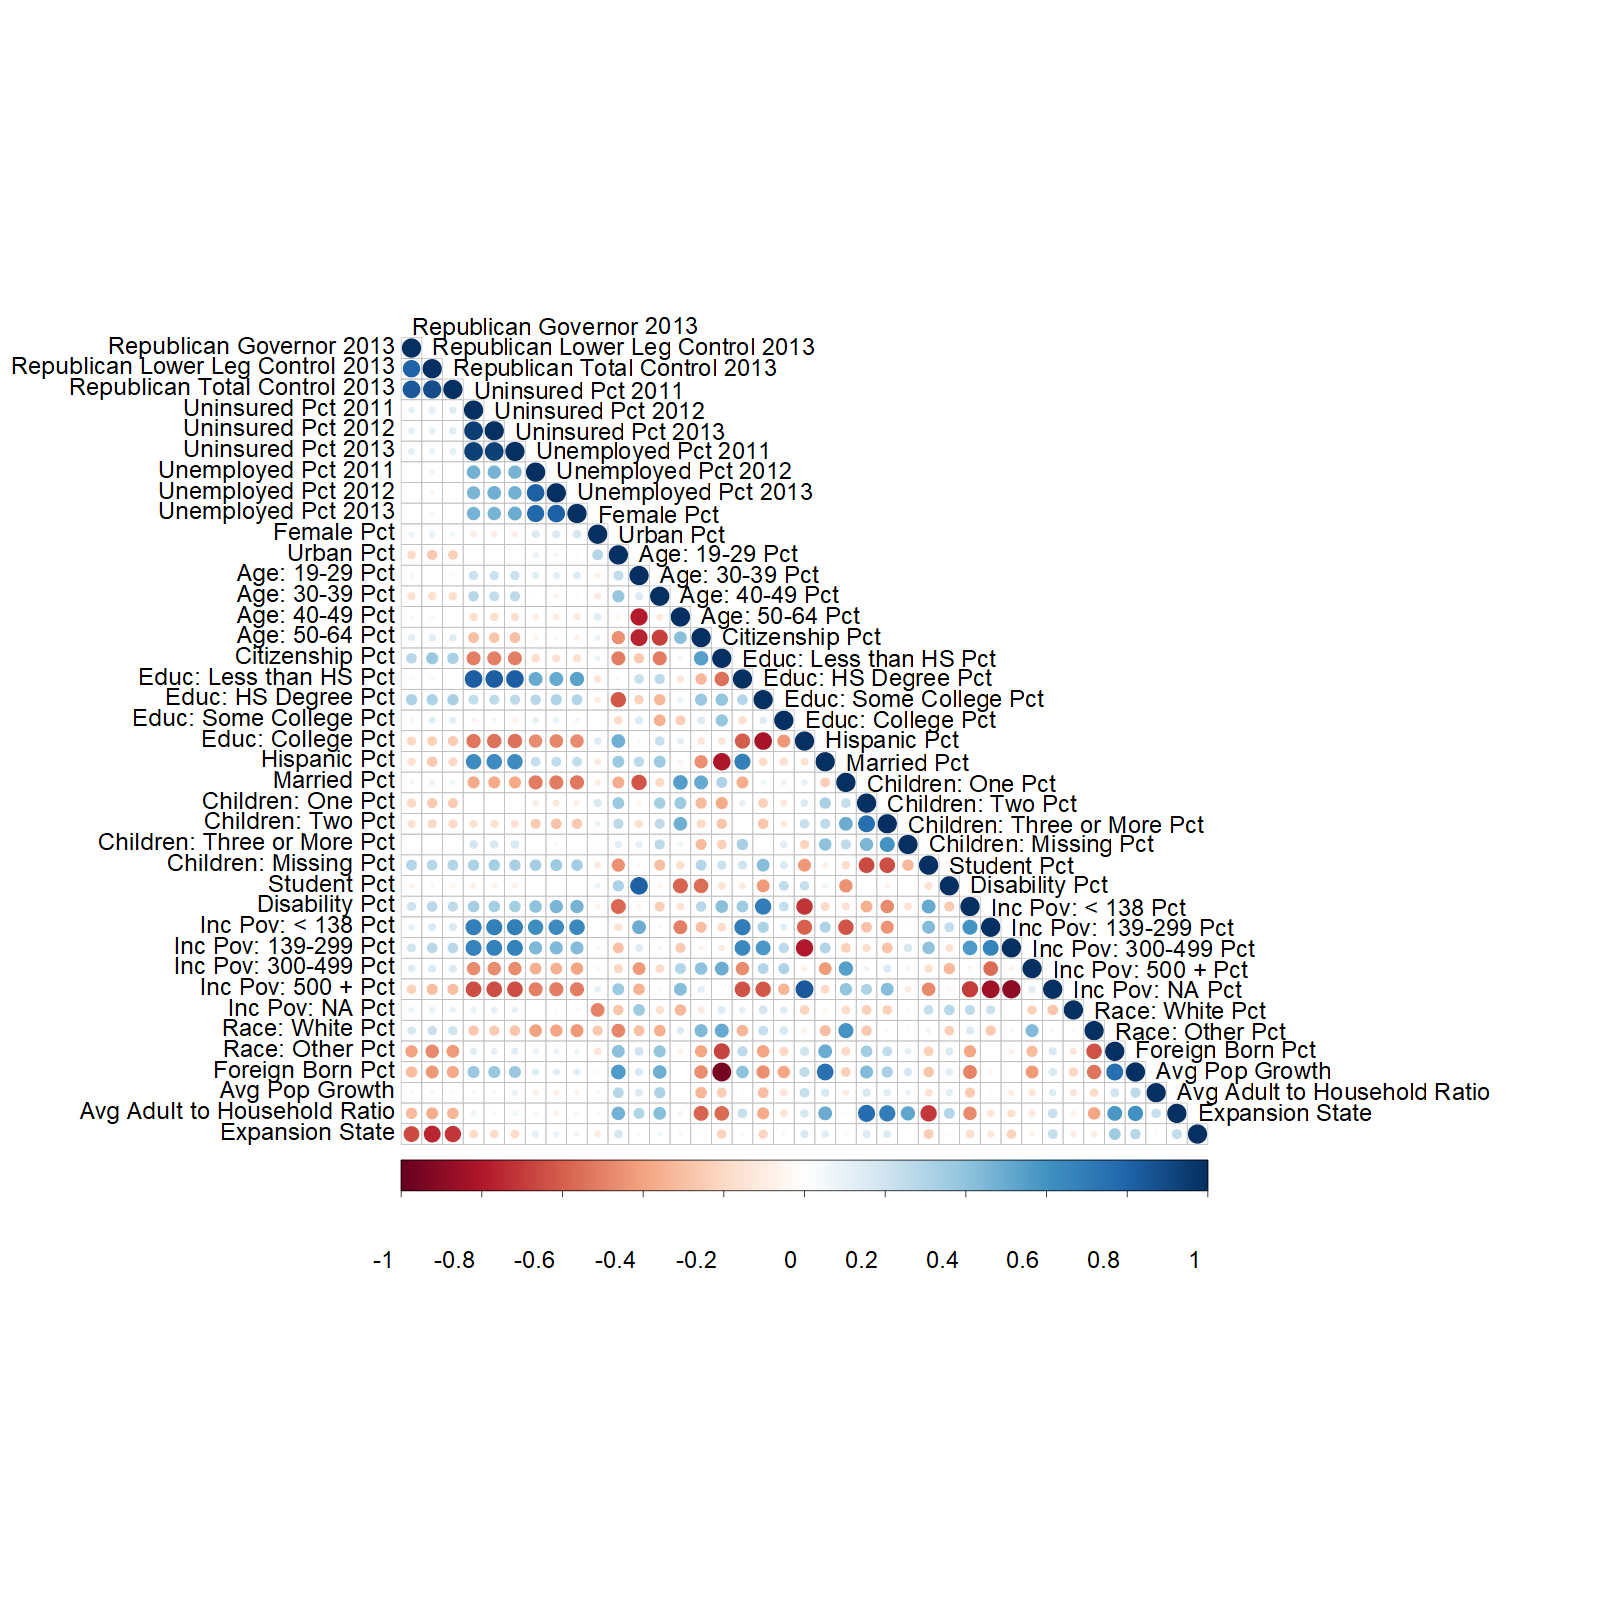
\includegraphics[scale=0.25]{01_Plots/correlation-plot-c1-sigma-zero.png}
\end{center}
\end{figure}

\clearpage

\begin{landscape}

\section{Weight Diagnostics}
\label{ssec:balancetables}

Table~\ref{tab:baltab1} displays the differences between the weighted mean covariate values of the expansion region and the mean of the non-expansion region for our primary dataset and with the early expansion states excluded (calculated using our the homogeneous covariate adjustments). The weights presented here are for the H-SBW estimator. The values under each column are in the following format: (unweighted difference, weighted difference). ``Primary'' and ``Early excluded'' refer to the primary dataset and those that exclude the early expansion states. ``Percent'' indicates that the differences displayed are in percentage points while ``Standardized'' indicates that the standardized mean differences are displayed. Additional results are available on request.

\begin{table}[h!]
\centering
    \caption{Balance table: percent and standardized mean differences, H-SBW weights}
    \label{tab:baltab1}
\begin{tabular}{lllll}
  \hline
Variables & Preferred (Percent) & Preferred (Standardized) & Early excluded (Percent) & Early excluded (Standardized) \\ 
  \hline
Age: 19-29 Pct & (-0.34, -0.34) & (-0.05, -0.05) & (-0.62, -0.21) & (-0.09, -0.03) \\ 
  Age: 30-39 Pct & (0.36, 0.17) & (0.1, 0.05) & (-0.04, 0.32) & (-0.01, 0.09) \\ 
  Age: 40-49 Pct & (0.19, -0.3) & (0.06, -0.1) & (-0.01, -0.44) & (0, -0.15) \\ 
  Avg Adult to Household Ratio & (11.29, -0.04) & (0.37, 0) & (3.37, 0.1) & (0.13, 0) \\ 
  Citizenship Pct & (-3.61, -1.59) & (-0.33, -0.15) & (-0.24, -1.45) & (-0.03, -0.16) \\ 
  Disability Pct & (-1.45, 0.52) & (-0.27, 0.1) & (-0.17, 0.63) & (-0.03, 0.11) \\ 
  Educ: HS Degree Pct & (-3.37, 0.54) & (-0.32, 0.05) & (-1.02, 0.64) & (-0.1, 0.06) \\ 
  Educ: Less than HS Pct & (-0.37, 0.83) & (-0.04, 0.1) & (-1.22, 0.76) & (-0.16, 0.1) \\ 
  Educ: Some College Pct & (-0.35, 0.4) & (-0.05, 0.06) & (0.36, 0.57) & (0.05, 0.08) \\ 
  Female Pct & (-0.34, -0.64) & (-0.16, -0.3) & (-0.25, -1) & (-0.12, -0.48) \\ 
  Foreign Born Pct & (7.6, 2) & (0.42, 0.11) & (1.02, 2) & (0.07, 0.13) \\ 
  Uninsured Pct 2011 & (-3.08, 0.05) & (-0.28, 0) & (-3.51, -0.05) & (-0.34, 0) \\ 
  Uninsured Pct 2012 & (-3, -0.05) & (-0.27, 0) & (-3.4, 0.05) & (-0.33, 0) \\ 
  Uninsured Pct 2013 & (-2.99, -0.05) & (-0.27, 0) & (-3.45, -0.05) & (-0.34, 0) \\ 
  Hispanic Pct & (4.46, 1) & (0.2, 0.04) & (-1.35, 1) & (-0.07, 0.05) \\ 
  Inc Pov: $<$ 138 Pct & (-2.05, 0.63) & (-0.19, 0.06) & (-1.33, 0.12) & (-0.12, 0.01) \\ 
  Inc Pov: 139-299 Pct & (-2.45, 0.65) & (-0.35, 0.09) & (-1.53, 0.5) & (-0.23, 0.08) \\ 
  Inc Pov: 300-499 Pct & (-0.59, -0.18) & (-0.12, -0.04) & (0.28, -0.18) & (0.06, -0.04) \\ 
  Inc Pov: 500 + Pct & (5.58, -1.3) & (0.35, -0.08) & (2.9, -1.23) & (0.2, -0.08) \\ 
  Married Pct & (-0.76, -0.43) & (-0.07, -0.04) & (-0.21, -0.53) & (-0.02, -0.05) \\ 
  Children: Missing Pct & (-3.25, -1) & (-0.36, -0.11) & (-1.99, -0.1) & (-0.21, -0.01) \\ 
  Children: One Pct & (0.7, -0.14) & (0.25, -0.05) & (0.11, -0.31) & (0.04, -0.12) \\ 
  Avg Pop Growth & (-0.09, -0.21) & (-0.07, -0.18) & (-0.26, -0.19) & (-0.22, -0.16) \\ 
  Race: White Pct & (-4.02, 1) & (-0.16, 0.04) & (0.09, 1) & (0, 0.04) \\ 
  Republican Governor 2013 & (-64.78, -25) & (-1.28, -0.5) & (-54.46, -24.87) & (-1.02, -0.47) \\ 
  Republican Lower Leg Control 2013 & (-74.72, -25) & (-1.69, -0.57) & (-56.67, -23.6) & (-1.12, -0.47) \\ 
  Republican Total Control 2013 & (-71.3, -25) & (-1.45, -0.51) & (-56.47, -25) & (-1.02, -0.45) \\ 
  Student Pct & (0.25, -0.5) & (0.04, -0.08) & (0.11, -0.25) & (0.02, -0.04) \\ 
  Children: Three or More Pct & (0, -0.21) & (0, -0.08) & (-0.17, -0.26) & (-0.07, -0.11) \\ 
  Children: Two Pct & (0.76, -0.31) & (0.23, -0.09) & (0.17, -0.37) & (0.05, -0.12) \\ 
  Unemployed Pct 2011 & (0.82, 0.15) & (0.18, 0.03) & (0.68, 0.15) & (0.15, 0.03) \\ 
  Unemployed Pct 2012 & (0.63, -0.03) & (0.14, -0.01) & (0.47, -0.03) & (0.11, -0.01) \\ 
  Unemployed Pct 2013 & (0.42, -0.15) & (0.11, -0.04) & (0.22, -0.15) & (0.06, -0.04) \\ 
  Urban Pct & (8.28, -2) & (0.26, -0.06) & (2.79, -2) & (0.08, -0.06) \\ 
   \hline
\end{tabular}
    \begin{tablenotes}
      \small
      \item The values displayed in each cell are the (weighted, unweighted) differences. The columns containing ``Standardized'' reflect the standardized mean differences while ``percent'' indicates the mean differences in percentage points. The columns containing ``Preferred'' indicate that this is for our primary analysis while ``Early excluded'' is for our analysis that excludes the early expansion states.
    \end{tablenotes}
\end{table}

Figure~\ref{fig:weightsbystatec2} display the weights summed by states when excluding the early expansion states for the H-SBW and BC-HSBW estimators.

\begin{figure}[H]
\begin{center}
    \caption{Total weights summed by state, early expansion removed}
    \label{fig:weightsbystatec2}
    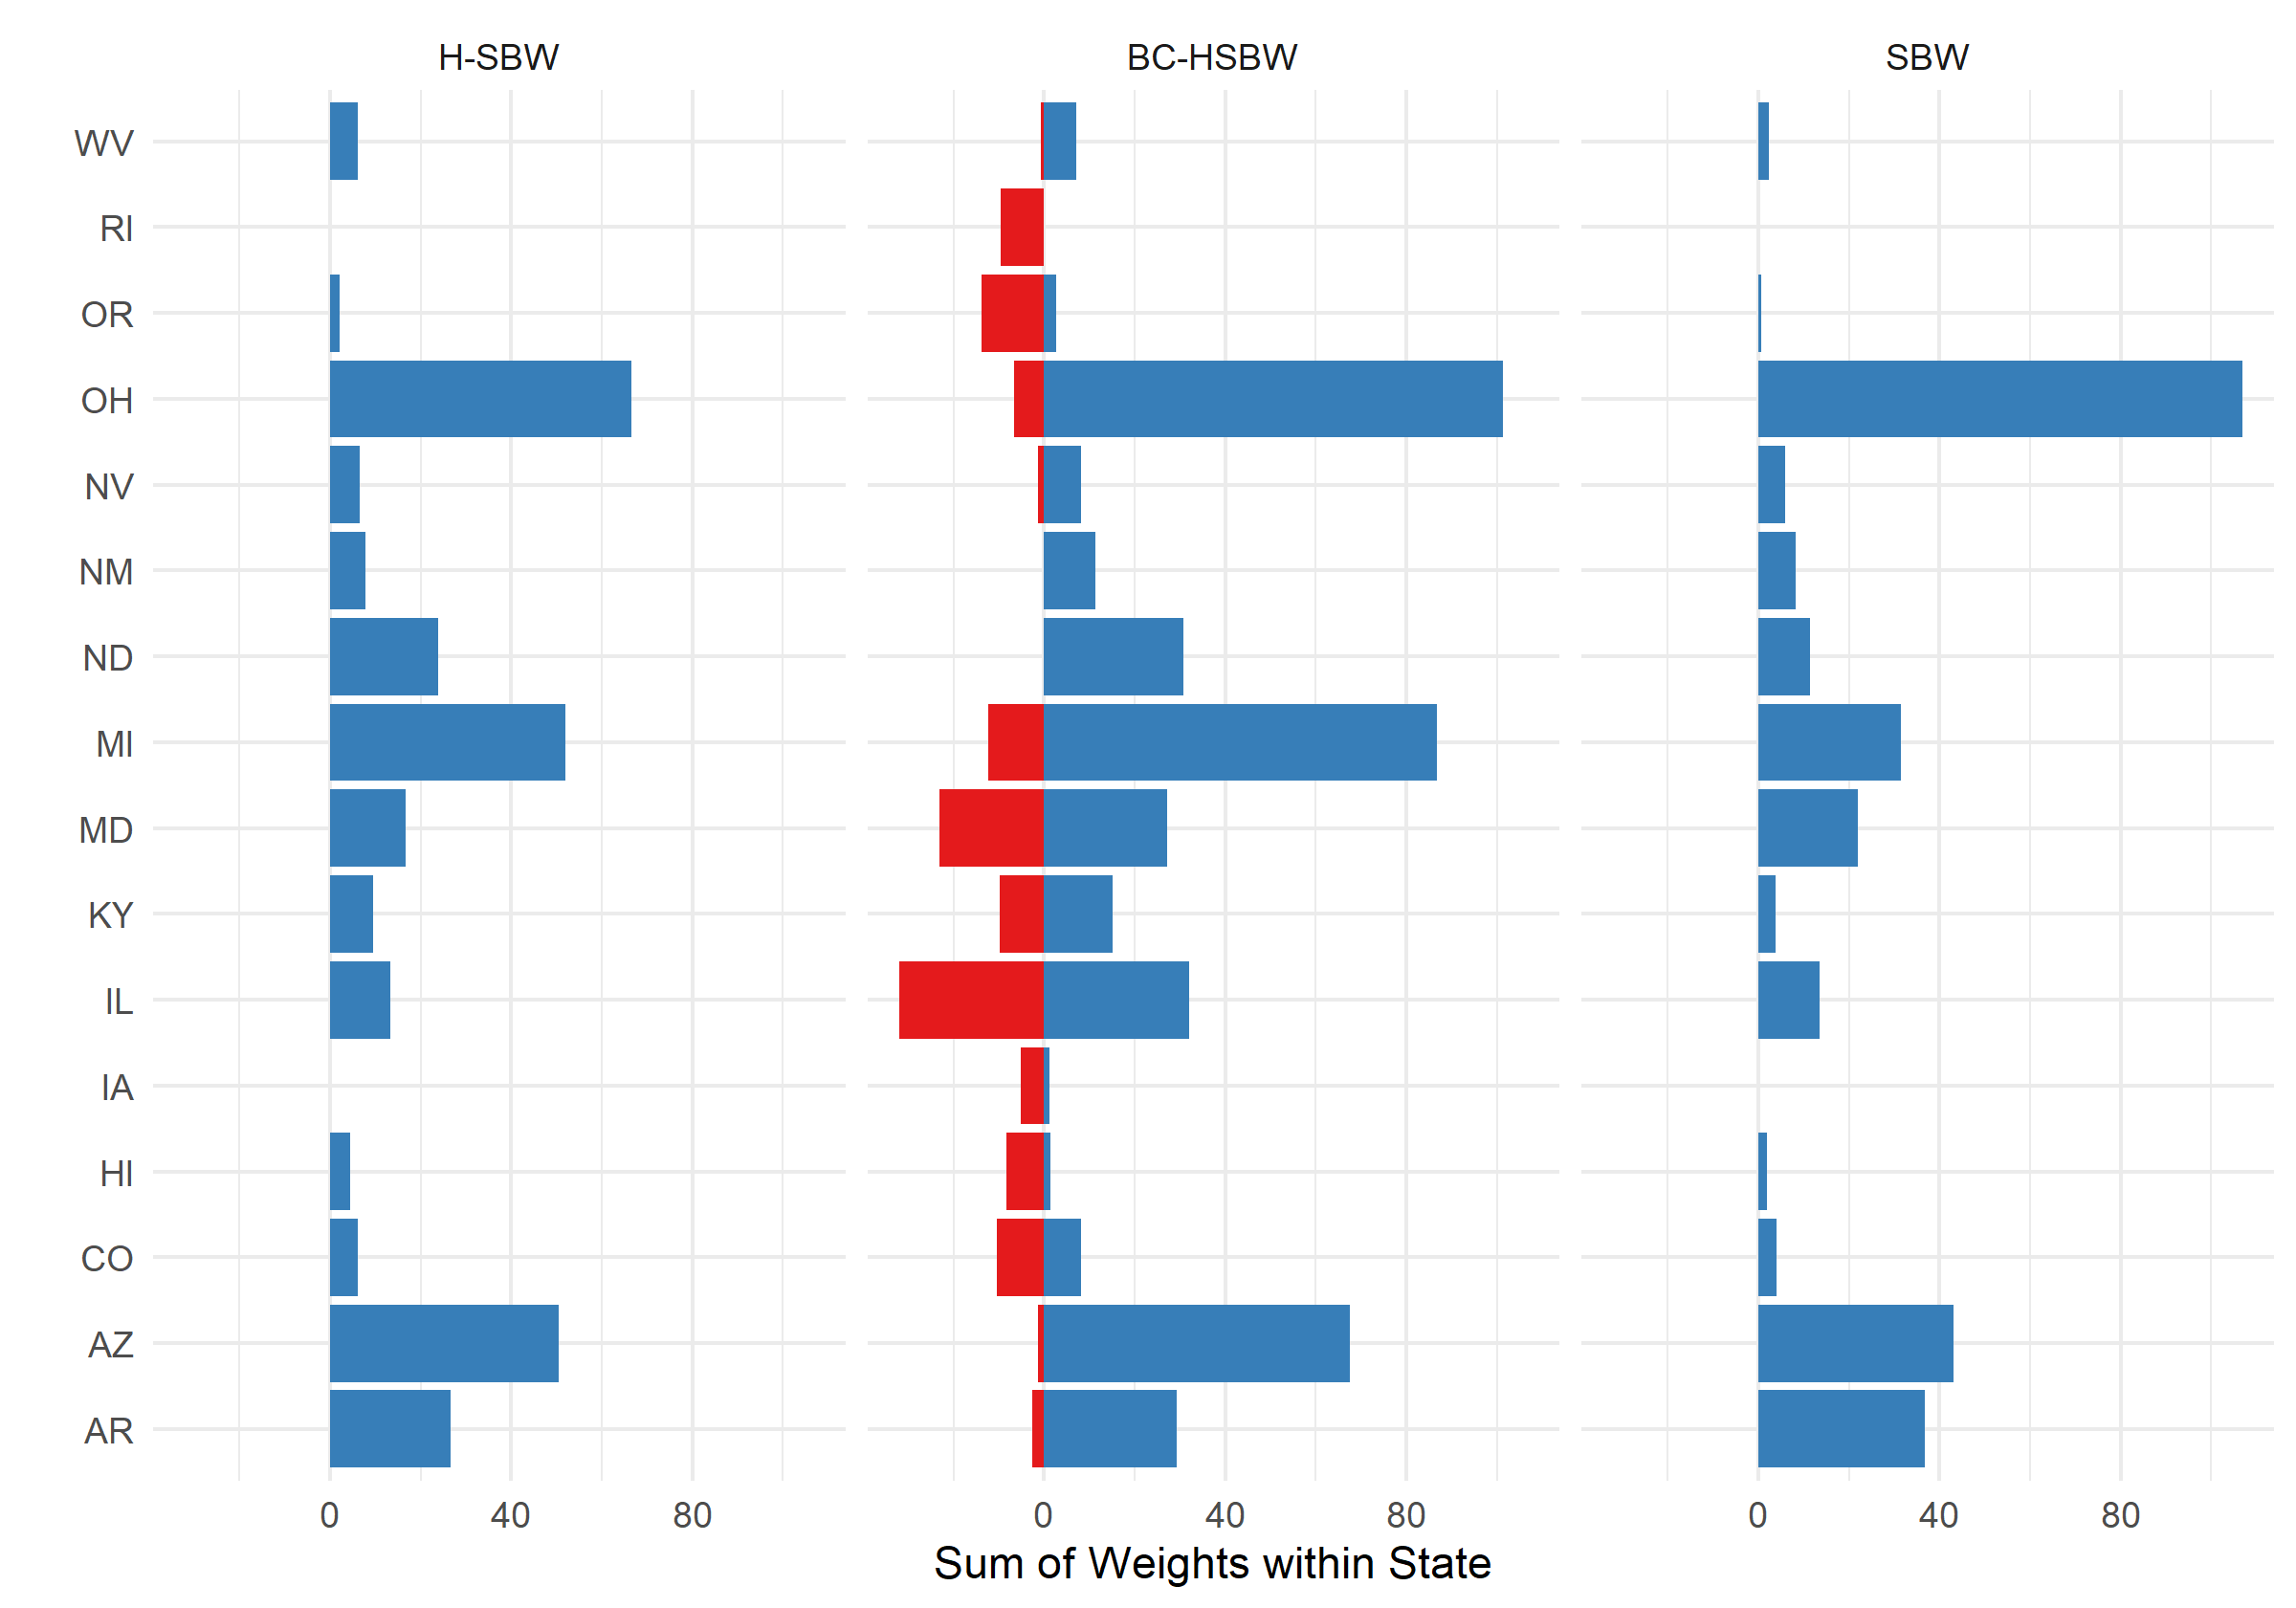
\includegraphics[scale=0.5]{01_Plots/weights-by-state-sbw-hsbw-c2-color.png}
\end{center}
\end{figure}
\end{landscape}
\clearpage

\section{Additional Results}
\label{ssec:allresults}

Table~\ref{tab:confintmain} displays the point estimates from all estimators as well as confidence intervals calculated either (a) leave-one-state-out jackknife on the adjusted dataset (CI (states)); (b) leave-one-state-out jackknife repeating the entire adjusted leaving each state out (CI (proc)). This table also includes all analyses calculated on a second version of the adjusted data where we use a common $\kappa$ for all values (sigma\_uu\_avg), which is the adjustment suggested by \cite{carroll2006measurement}. Notice that the confidence intervals are identical for ``sigma\_zero'' because this is the unadjusted dataset. ``sigma\_uu\_i'' is our preferred covariate adjustment.

\begin{table}[ht]
\centering
\caption{Point estimates and confidence intervals, primary dataset}
\label{tab:confintmain}
\begin{tabular}{llrll}
  \hline
Weight type & Sigma estimate & Psihat & CI (states) & CI (proc) \\ 
  \hline
H-SBW & sigma\_uu\_i & -2.17 & (-3.41, -0.94) & (-3.42, -0.92) \\ 
  H-SBW & sigma\_uu\_avg & -2.25 & (-3.51, -0.99) & (-3.35, -1.14) \\ 
  H-SBW & sigma\_zero & -2.35 & (-3.09, -1.61) & (-3.09, -1.61) \\ 
  BC-HSBW & sigma\_uu\_i & -2.13 & (-3.55, -0.71) & (-3.42, -0.84) \\ 
  BC-HSBW & sigma\_uu\_avg & -2.17 & (-3.57, -0.78) & (-3.39, -0.96) \\ 
  BC-HSBW & sigma\_zero & -2.40 & (-3.33, -1.46) & (-3.33, -1.46) \\ 
  SBW & sigma\_uu\_i & -2.24 & (-3.50, -0.99) & (-3.51, -0.97) \\ 
  SBW & sigma\_uu\_avg & -2.30 & (-3.67, -0.92) & (-3.45, -1.15) \\ 
  SBW & sigma\_zero & -2.40 & (-3.10, -1.69) & (-3.10, -1.69) \\ 
  BC-SBW & sigma\_uu\_i & -2.12 & (-3.15, -1.10) & (-3.11, -1.14) \\ 
  BC-SBW & sigma\_uu\_avg & -2.17 & (-3.25, -1.08) & (-3.22, -1.12) \\ 
  BC-SBW & sigma\_zero & -2.36 & (-2.93, -1.80) & (-2.93, -1.80) \\ 
   \hline
\end{tabular}
\end{table}

Table~\ref{tab:ptests} presents all point estimates from estimators that we calculated. The ``Var subset`` column indicates which variables were excluded from the estimation: 0 excludes no variables; 1 removes Republican governance indicators; 2 pre-treatment uninsurance and unemployment rates; 3 urban, age, education, citizenship, marital status, student, disability, or female; 4 race, ethnicity, income, foreign born; 5 children, population growth, and household to person ratio. We see that the largest changes generally occur when excluding the pre-treatment uninsurance and unemployment rates. This is not surprising: controlling for the other covariates, the pre-treatment uninsurance rate was substantially lower in the treated region compared to the control region. Given that pre-treatment uninsurance rates are highly correlated with post-treatment rates, we find that this comparison leads to a larger absolute magnitude point estimate, highlighting the need to control for these covariates.

%Wed Jan 13 15:24:43 2021
\begin{table}[ht]
\centering
\caption{Point estimates for all specifications}
\label{tab:ptests}
\begin{tabular}{rlrrrr}
  \hline
Variable subset & Sigma estimate & H-SBW & BC-HSBW & SBW & BC-SBW \\ 
  \hline
0 & sigma\_uu\_i & -2.17 & -2.13 & -2.24 & -2.12 \\ 
  0 & sigma\_uu\_avg & -2.25 & -2.17 & -2.30 & -2.17 \\ 
  0 & sigma\_zero & -2.35 & -2.40 & -2.40 & -2.36 \\ 
  1 & sigma\_uu\_i & -2.85 & -2.87 & -3.00 & -2.76 \\ 
  1 & sigma\_uu\_avg & -2.86 & -2.86 & -2.99 & -2.75 \\ 
  1 & sigma\_zero & -3.00 & -3.09 & -3.07 & -2.92 \\ 
  2 & sigma\_uu\_i & -5.73 & -5.05 & -5.24 & -4.70 \\ 
  2 & sigma\_uu\_avg & -5.73 & -5.05 & -5.24 & -4.70 \\ 
  2 & sigma\_zero & -5.73 & -5.13 & -5.24 & -4.77 \\ 
  3 & sigma\_uu\_i & -2.17 & -2.00 & -2.24 & -2.00 \\ 
  3 & sigma\_uu\_avg & -2.25 & -2.06 & -2.29 & -2.06 \\ 
  3 & sigma\_zero & -2.34 & -2.17 & -2.40 & -2.15 \\ 
  4 & sigma\_uu\_i & -2.35 & -2.39 & -2.29 & -2.30 \\ 
  4 & sigma\_uu\_avg & -2.39 & -2.39 & -2.32 & -2.32 \\ 
  4 & sigma\_zero & -2.45 & -2.59 & -2.43 & -2.49 \\ 
  5 & sigma\_uu\_i & -2.17 & -2.19 & -2.26 & -2.21 \\ 
  5 & sigma\_uu\_avg & -2.25 & -2.24 & -2.33 & -2.27 \\ 
  5 & sigma\_zero & -2.35 & -2.44 & -2.42 & -2.47 \\ 
   \hline
\end{tabular}
\end{table}

Table ~\ref{tab:confintmainc2} and Table~\ref{tab:secondaryptests} are identical to the structure of the previous two tables except we exclude the ``early expansion states'' from the pool of expansion state matches. 

\begin{table}[ht]
\centering
\caption{Point estimates and confidence intervals, early expansion excluded}
\label{tab:confintmainc2}
\begin{tabular}{llrll}
  \hline
Weight type & Sigma estimate & Psihat & CI (states) & CI (proc) \\ 
  \hline
H-SBW & sigma\_uu\_i & -2.05 & (-3.10, -1.00) & (-3.05, -1.05) \\ 
  H-SBW & sigma\_uu\_avg & -2.13 & (-3.20, -1.05) & (-3.17, -1.08) \\ 
  H-SBW & sigma\_zero & -2.29 & (-2.90, -1.69) & (-2.90, -1.69) \\ 
  BC-HSBW & sigma\_uu\_i & -2.14 & (-3.63, -0.64) & (-3.48, -0.80) \\ 
  BC-HSBW & sigma\_uu\_avg & -2.19 & (-3.65, -0.73) & (-3.57, -0.81) \\ 
  BC-HSBW & sigma\_zero & -2.50 & (-3.66, -1.33) & (-3.66, -1.33) \\ 
  SBW & sigma\_uu\_i & -1.91 & (-2.91, -0.91) & (-2.79, -1.03) \\ 
  SBW & sigma\_uu\_avg & -2.01 & (-3.02, -1.00) & (-2.83, -1.19) \\ 
  SBW & sigma\_zero & -2.20 & (-2.69, -1.71) & (-2.69, -1.71) \\ 
  BC-SBW & sigma\_uu\_i & -1.97 & (-3.49, -0.44) & (-3.27, -0.66) \\ 
  BC-SBW & sigma\_uu\_avg & -2.04 & (-3.59, -0.50) & (-3.39, -0.70) \\ 
  BC-SBW & sigma\_zero & -2.34 & (-3.44, -1.25) & (-3.44, -1.25) \\ 
   \hline
\end{tabular}
\end{table}

\begin{table}[ht]
\centering
   \caption{Point estimates for all specifications, early expansion excluded}
    \label{tab:secondaryptests}
\begin{tabular}{rlrrrr}
  \hline
Variable subset & Sigma estimate & H-SBW & BC-HSBW & SBW & BC-SBW \\ 
  \hline
0 & sigma\_uu\_i & -2.05 & -2.14 & -1.91 & -1.97 \\ 
  0 & sigma\_uu\_avg & -2.13 & -2.19 & -2.01 & -2.04 \\ 
  0 & sigma\_zero & -2.29 & -2.50 & -2.20 & -2.34 \\ 
  1 & sigma\_uu\_i & -2.85 & -2.99 & -2.85 & -2.86 \\ 
  1 & sigma\_uu\_avg & -2.86 & -2.98 & -2.86 & -2.86 \\ 
  1 & sigma\_zero & -3.05 & -3.18 & -2.96 & -2.99 \\ 
  2 & sigma\_uu\_i & -5.55 & -4.46 & -5.02 & -4.52 \\ 
  2 & sigma\_uu\_avg & -5.55 & -4.73 & -5.01 & -4.53 \\ 
  2 & sigma\_zero & -5.55 & -4.78 & -5.01 & -4.56 \\ 
  3 & sigma\_uu\_i & -2.05 & -2.03 & -1.91 & -1.89 \\ 
  3 & sigma\_uu\_avg & -2.13 & -2.10 & -2.00 & -1.97 \\ 
  3 & sigma\_zero & -2.27 & -2.22 & -2.20 & -2.13 \\ 
  4 & sigma\_uu\_i & -2.27 & -2.24 & -2.15 & -2.00 \\ 
  4 & sigma\_uu\_avg & -2.35 & -2.28 & -2.23 & -2.04 \\ 
  4 & sigma\_zero & -2.36 & -2.62 & -2.28 & -2.45 \\ 
  5 & sigma\_uu\_i & -2.05 & -2.20 & -1.91 & -2.03 \\ 
  5 & sigma\_uu\_avg & -2.13 & -2.26 & -1.99 & -2.11 \\ 
  5 & sigma\_zero & -2.29 & -2.45 & -2.19 & -2.36 \\ 
   \hline
\end{tabular}
\end{table}

Table~\ref{tab:loostatec1} and Table~\ref{tab:loostatec2} present point estimates for the leave-one-state out analysis for our preferred estimator, H-SBW calculated on our preferred covariate adjustment for the primary dataset and when excluding early expansion states.

\begin{table}[ht]
\centering
   \caption{Leave-one-state-out point estimates, primary dataset, preferred adjustment}
    \label{tab:loostatec1}
\begin{tabular}{lrlrl}
  \hline
State & Psihat (0) & None (states, proc) & Psihat (1) & Repub (states, proc) \\ 
  \hline
AR & -2.17 & (-2.34, -2.38) & -2.85 & (-2.81, -2.80) \\ 
  AZ & -2.17 & (-2.21, -2.24) & -2.85 & (-2.86, -2.86) \\ 
  CA & -2.17 & (-1.99, -2.02) & -2.85 & (-2.77, -2.76) \\ 
  CO & -2.17 & (-2.17, -2.23) & -2.85 & (-2.84, -2.84) \\ 
  CT & -2.17 & (-2.17, -2.15) & -2.85 & (-2.83, -2.82) \\ 
  HI & -2.17 & (-2.15, -2.14) & -2.85 & (-2.77, -2.78) \\ 
  IA & -2.17 & (-2.09, -2.07) & -2.85 & (-2.83, -2.84) \\ 
  IL & -2.17 & (-2.16, -2.24) & -2.85 & (-2.83, -2.84) \\ 
  KY & -2.17 & (-2.02, -1.95) & -2.85 & (-2.57, -2.52) \\ 
  MD & -2.17 & (-2.25, -2.27) & -2.85 & (-2.94, -2.94) \\ 
  MI & -2.17 & (-2.10, -2.18) & -2.85 & (-2.89, -2.92) \\ 
  MN & -2.17 & (-2.17, -2.19) & -2.85 & (-2.84, -2.86) \\ 
  ND & -2.17 & (-2.23, -2.26) & -2.85 & (-2.84, -2.84) \\ 
  NH & -2.17 & (-2.18, -2.21) & -2.85 & (-2.98, -2.99) \\ 
  NJ & -2.17 & (-2.26, -2.25) & -2.85 & (-2.99, -3.03) \\ 
  NM & -2.17 & (-2.16, -2.22) & -2.85 & (-2.76, -2.77) \\ 
  NV & -2.17 & (-2.21, -2.24) & -2.85 & (-2.89, -2.88) \\ 
  OH & -2.17 & (-2.70, -2.68) & -2.85 & (-3.00, -2.98) \\ 
  OR & -2.17 & (-2.17, -2.25) & -2.85 & (-2.80, -2.84) \\ 
  RI & -2.17 & (-2.17, -2.15) & -2.85 & (-2.81, -2.81) \\ 
  WA & -2.17 & (-2.10, -2.11) & -2.85 & (-2.78, -2.77) \\ 
  WV & -2.17 & (-2.16, -2.18) & -2.85 & (-2.8, -2.78) \\ 
   \hline
\end{tabular}
\end{table}

\begin{table}[ht]
\centering
   \caption{Leave-one-state-out point estimates, early expansion excluded, preferred adjustment}
    \label{tab:loostatec2}
\begin{tabular}{lrlrl}
  \hline
State & Psihat (0) & None (states, proc) & Psihat (1) & Repub (states, proc) \\ 
  \hline
AR & -2.05 & (-2.15, -2.16) & -2.85 & (-2.77, -2.76) \\ 
  AZ & -2.05 & (-1.82, -1.88) & -2.85 & (-2.87, -2.86) \\ 
  CO & -2.05 & (-2.07, -2.09) & -2.85 & (-2.84, -2.83) \\ 
  HI & -2.05 & (-2.01, -1.99) & -2.85 & (-2.71, -2.73) \\ 
  IA & -2.05 & (-1.98, -1.95) & -2.85 & (-2.85, -2.86) \\ 
  IL & -2.05 & (-2.03, -2.01) & -2.85 & (-2.8, -2.79) \\ 
  KY & -2.05 & (-1.87, -1.8) & -2.85 & (-2.59, -2.54) \\ 
  MD & -2.05 & (-2.18, -2.15) & -2.85 & (-2.97, -2.96) \\ 
  MI & -2.05 & (-1.96, -2) & -2.85 & (-2.92, -2.96) \\ 
  ND & -2.05 & (-2.02, -2.04) & -2.85 & (-2.84, -2.84) \\ 
  NH & -2.05 & (-2.05, -2.06) & -2.85 & (-3.02, -3.03) \\ 
  NM & -2.05 & (-1.99, -1.97) & -2.85 & (-2.72, -2.75) \\ 
  NV & -2.05 & (-2.15, -2.15) & -2.85 & (-2.93, -2.92) \\ 
  OH & -2.05 & (-2.43, -2.38) & -2.85 & (-3.03, -3.02) \\ 
  OR & -2.05 & (-2.05, -2.11) & -2.85 & (-2.81, -2.84) \\ 
  RI & -2.05 & (-2.05, -2.05) & -2.85 & (-2.80, -2.80) \\ 
  WV & -2.05 & (-2.06, -2.06) & -2.85 & (-2.83, -2.81) \\ 
   \hline
\end{tabular}
\end{table}

Table~\ref{tab:oateconfint} displays point estimates and confidence intervals for the primary point estimates for the OATE. We display the confidence intervals calculated using both the leave-one-out-states conditional on the covariate adjustment (CI (states)) and recalculating the covariate adjustment for the OATE (CI (proc)). 

\begin{table}[ht]
\centering
\caption{OATE primary results inference}
\label{tab:oateconfint}
\begin{tabular}{rllll}
  \hline
Psihat & Sigma estimate & Dataset & CI (states) & CI (proc) \\ 
  \hline
-1.74 & sigma\_uu\_i\_modeled & c1 & (-2.35, -1.14) & (-2.48, -1.00) \\ 
  -1.67 & sigma\_uu\_avg & c1 & (-2.34, -0.99) & (-2.52, -0.81) \\ 
  -1.80 & sigma\_zero & c1 & (-2.50, -1.10) & (-2.50, -1.10) \\ 
  -1.89 & sigma\_uu\_i\_modeled & c2 & (-2.47, -1.32) & (-2.54, -1.24) \\ 
  -1.80 & sigma\_uu\_avg & c2 & (-2.43, -1.17) & (-2.57, -1.03) \\ 
  -1.95 & sigma\_zero & c2 & (-2.65, -1.25) & (-2.65, -1.25) \\ 
   \hline
\end{tabular}
\end{table}

Table~\ref{tab:oatesensitive} presents all point estimates calculate using the overlap weights. Dataset ``c1'' refers to the primary dataset and dataset ``c2'' removes the early expansion states. The numeric column names refer to the covariate group excluded (covariate groups described above).

\begin{table}[ht]
\centering
\caption{OATE all point estimates}
\label{tab:oatesensitive}
\begin{tabular}{llrrrrrr}
  \hline
Sigma estimate & Dataset & 0 & 1 & 2 & 3 & 4 & 5 \\ 
  \hline
sigma\_uu\_i & c1 & -1.64 & -2.60 & -2.96 & -1.86 & -1.86 & -1.77 \\ 
  sigma\_uu\_i & c2 & -1.81 & -2.53 & -3.10 & -2.18 & -2.04 & -1.96 \\ 
  sigma\_avg & c1 & -1.58 & -2.62 & -2.85 & -1.76 & -1.76 & -1.78 \\ 
  sigma\_avg & c2 & -1.74 & -2.54 & -3.00 & -2.10 & -1.96 & -1.95 \\ 
  sigma\_zero & c1 & -1.80 & -2.55 & -3.11 & -1.98 & -1.94 & -1.83 \\ 
  sigma\_zero & c2 & -1.95 & -2.51 & -3.25 & -2.12 & -2.10 & -2.00 \\ 
   \hline
\end{tabular}
\end{table}

Table~\ref{tab:rdiffc1} and ~\ref{tab:rdiffc2} display the quantiles of the distribution $\hat{\Delta}_v^1$ estimates when leaving out each state for the primary dataset and removing the early expansion states. The ``resample'' column indicates whether the entire adjustment procedure was recalculated (``proc'') or whether we left out each state conditional on the adjustment (``states''). Table~\ref{tab:hte} displays the estimated linear combination of model coefficients on the Republican governance indicators with 95 percent confidence intervals (standard errors clustered at the state level). The ``Weights'' column represents whether the regressions were weighted; we ran two versions, an unweighted regression and one using the overlap weights.

\begin{table}[ht]
\centering
\label{tab:rdiffc1}
\caption{$\hat{\Delta}^1_v$ leave-one-state-out estimates, primary dataset}
\begin{tabular}{lllrrrrrr}
  \hline
Resample & Sigma estimate & Weight type & Original & 0\% & 25\% & 50\% & 75\% & 100\% \\ 
  \hline
states & sigma\_uu\_i\_modeled & H-SBW & -0.67 & -0.80 & -0.68 & -0.67 & -0.62 & -0.30 \\ 
  proc & sigma\_uu\_i\_modeled & H-SBW & -0.67 & -0.78 & -0.68 & -0.64 & -0.59 & -0.30 \\ 
  states & sigma\_uu\_i\_modeled & BC-HSBW & -0.74 & -0.87 & -0.77 & -0.71 & -0.69 & -0.26 \\ 
  proc & sigma\_uu\_i\_modeled & BC-HSBW & -0.74 & -0.85 & -0.76 & -0.70 & -0.67 & -0.34 \\ 
  states & sigma\_uu\_i\_modeled & SBW & -0.75 & -0.98 & -0.77 & -0.75 & -0.72 & -0.48 \\ 
  proc & sigma\_uu\_i\_modeled & SBW & -0.75 & -0.98 & -0.78 & -0.73 & -0.67 & -0.49 \\ 
  states & sigma\_uu\_i\_modeled & BC-SBW & -0.63 & -0.85 & -0.69 & -0.62 & -0.61 & -0.39 \\ 
  proc & sigma\_uu\_i\_modeled & BC-SBW & -0.63 & -0.82 & -0.68 & -0.64 & -0.59 & -0.35 \\ 
  states & sigma\_uu\_avg & H-SBW & -0.61 & -0.74 & -0.64 & -0.60 & -0.57 & -0.23 \\ 
  proc & sigma\_uu\_avg & H-SBW & -0.61 & -0.76 & -0.63 & -0.59 & -0.55 & -0.33 \\ 
  states & sigma\_uu\_avg & BC-HSBW & -0.69 & -0.83 & -0.73 & -0.68 & -0.64 & -0.24 \\ 
  proc & sigma\_uu\_avg & BC-HSBW & -0.69 & -0.83 & -0.73 & -0.66 & -0.63 & -0.39 \\ 
  states & sigma\_uu\_avg & SBW & -0.70 & -0.89 & -0.72 & -0.69 & -0.67 & -0.31 \\ 
  proc & sigma\_uu\_avg & SBW & -0.70 & -0.93 & -0.73 & -0.68 & -0.65 & -0.49 \\ 
  states & sigma\_uu\_avg & BC-SBW & -0.58 & -0.78 & -0.63 & -0.57 & -0.56 & -0.32 \\ 
  proc & sigma\_uu\_avg & BC-SBW & -0.58 & -0.81 & -0.63 & -0.58 & -0.55 & -0.28 \\ 
  states & sigma\_zero & H-SBW & -0.65 & -0.78 & -0.66 & -0.63 & -0.61 & -0.50 \\ 
  proc & sigma\_zero & H-SBW & -0.65 & -0.78 & -0.66 & -0.63 & -0.61 & -0.50 \\ 
  states & sigma\_zero & BC-HSBW & -0.70 & -0.88 & -0.74 & -0.68 & -0.64 & -0.50 \\ 
  proc & sigma\_zero & BC-HSBW & -0.70 & -0.88 & -0.74 & -0.68 & -0.64 & -0.50 \\ 
  states & sigma\_zero & SBW & -0.68 & -0.84 & -0.71 & -0.68 & -0.66 & -0.49 \\ 
  proc & sigma\_zero & SBW & -0.68 & -0.84 & -0.71 & -0.68 & -0.66 & -0.49 \\ 
  states & sigma\_zero & BC-SBW & -0.56 & -0.67 & -0.61 & -0.55 & -0.52 & -0.39 \\ 
  proc & sigma\_zero & BC-SBW & -0.56 & -0.67 & -0.61 & -0.55 & -0.52 & -0.39 \\ 
   \hline
\end{tabular}
\end{table}

\begin{table}[ht]
\label{tab:rdiffc2}
\caption{$\hat{\Delta}^1_v$ leave-one-state-out estimates, early expansion excluded}
\centering
\begin{tabular}{lllrrrrrr}
  \hline
Resample & Sigma estimate & Weight type & Original & 0\% & 25\% & 50\% & 75\% & 100\% \\ 
  \hline
states & sigma\_uu\_i\_modeled & H-SBW & -0.80 & -1.05 & -0.82 & -0.77 & -0.73 & -0.60 \\ 
  proc & sigma\_uu\_i\_modeled & H-SBW & -0.80 & -0.98 & -0.81 & -0.76 & -0.74 & -0.60 \\ 
  states & sigma\_uu\_i\_modeled & BC-HSBW & -0.85 & -1.13 & -0.96 & -0.83 & -0.76 & -0.45 \\ 
  proc & sigma\_uu\_i\_modeled & BC-HSBW & -0.85 & -1.05 & -0.94 & -0.83 & -0.77 & -0.53 \\ 
  states & sigma\_uu\_i\_modeled & SBW & -0.94 & -1.15 & -0.94 & -0.92 & -0.89 & -0.70 \\ 
  proc & sigma\_uu\_i\_modeled & SBW & -0.94 & -1.05 & -0.98 & -0.91 & -0.86 & -0.73 \\ 
  states & sigma\_uu\_i\_modeled & BC-SBW & -0.89 & -1.27 & -0.93 & -0.86 & -0.81 & -0.26 \\ 
  proc & sigma\_uu\_i\_modeled & BC-SBW & -0.89 & -1.19 & -0.96 & -0.86 & -0.81 & -0.37 \\ 
  states & sigma\_uu\_avg & H-SBW & -0.73 & -0.99 & -0.74 & -0.70 & -0.68 & -0.51 \\ 
  proc & sigma\_uu\_avg & H-SBW & -0.73 & -0.94 & -0.73 & -0.69 & -0.67 & -0.50 \\ 
  states & sigma\_uu\_avg & BC-HSBW & -0.79 & -1.10 & -0.87 & -0.78 & -0.69 & -0.42 \\ 
  proc & sigma\_uu\_avg & BC-HSBW & -0.79 & -1.01 & -0.89 & -0.73 & -0.69 & -0.46 \\ 
  states & sigma\_uu\_avg & SBW & -0.85 & -1.08 & -0.85 & -0.83 & -0.81 & -0.66 \\ 
  proc & sigma\_uu\_avg & SBW & -0.85 & -0.95 & -0.86 & -0.82 & -0.80 & -0.68 \\ 
  states & sigma\_uu\_avg & BC-SBW & -0.82 & -1.21 & -0.86 & -0.80 & -0.74 & -0.18 \\ 
  proc & sigma\_uu\_avg & BC-SBW & -0.82 & -1.09 & -0.86 & -0.76 & -0.74 & -0.26 \\ 
  states & sigma\_zero & H-SBW & -0.76 & -0.95 & -0.83 & -0.74 & -0.70 & -0.58 \\ 
  proc & sigma\_zero & H-SBW & -0.76 & -0.95 & -0.83 & -0.74 & -0.70 & -0.58 \\ 
  states & sigma\_zero & BC-HSBW & -0.69 & -1.00 & -0.83 & -0.70 & -0.60 & -0.39 \\ 
  proc & sigma\_zero & BC-HSBW & -0.69 & -1.00 & -0.83 & -0.70 & -0.60 & -0.39 \\ 
  states & sigma\_zero & SBW & -0.76 & -0.91 & -0.83 & -0.75 & -0.74 & -0.51 \\ 
  proc & sigma\_zero & SBW & -0.76 & -0.91 & -0.83 & -0.75 & -0.74 & -0.51 \\ 
  states & sigma\_zero & BC-SBW & -0.64 & -1.06 & -0.70 & -0.58 & -0.55 & -0.38 \\ 
  proc & sigma\_zero & BC-SBW & -0.64 & -1.06 & -0.70 & -0.58 & -0.55 & -0.38 \\ 
   \hline
\end{tabular}
\end{table}

\begin{table}[ht]
\caption{OLS HTE estimates}
\label{tab:hte}
\centering
\begin{tabular}{rllll}
  \hline
Estimate & Dataset & Sigma estimate & CI 95 & Weights \\ 
  \hline
  -1.76 & c1 & sigma\_uu\_i\_modeled & (-5.47, 1.94) & Overlap \\ 
  -1.67 & c1 & sigma\_uu\_avg & (-7.18, 3.84) & Overlap \\ 
  -1.97 & c1 & sigma\_zero & (-4.11, 0.17) & Overlap \\ 
  0.51 & c2 & sigma\_uu\_i\_modeled & (-6.00, 7.02) & Overlap \\ 
  -0.17 & c2 & sigma\_uu\_avg & (-8.17, 7.83) & Overlap \\ 
  -1.48 & c2 & sigma\_zero & (-3.51, 0.54) & Overlap \\ 
  0.10 & c1 & sigma\_uu\_i\_modeled & (-1.09, 1.30) & None \\ 
  0.61 & c1 & sigma\_uu\_avg & (-1.82, 3.04) & None \\ 
  -0.12 & c1 & sigma\_zero & (-0.90, 0.66) & None \\ 
  0.37 & c2 & sigma\_uu\_i\_modeled & (-0.9, 1.63) & None \\ 
  0.64 & c2 & sigma\_uu\_avg & (-1.77, 3.04) & None \\ 
  -0.11 & c2 & sigma\_zero & (-0.91, 0.68) & None \\ 
   \hline
\end{tabular}
\end{table}


\end{appendix}

\end{document}